\chapter{OTA - Exercício 2 - Analíticos} \label{Chap:AppendixAnaliticosA02}

%CASO 1
\begin{xltabular}{\textwidth}{|l|X|X|}
	\hline
	\endfirsthead
	
	\hline \multicolumn{3}{|c|}{continuação da página anterior} \\ \hline
	\endhead
	
	\hline \multicolumn{3}{|r|}{Continua na próxima página} \\ \hline
	\endfoot
	
	\hline
	\endlastfoot
	
	\multicolumn{3}{|c|}{\cellcolor[HTML]{C0C0C0}\textbf{CASO DE TESTE 1}} \\ \hline

	%EF1
	\multicolumn{3}{|c|}{\cellcolor[HTML]{DEDEDE}\textbf{Nota Ponderada - EF1}} \\ \hline
	\multicolumn{3}{|c|}{\textbf{Blocos}} \\ \hline
	\multicolumn{3}{|l|}{\begin{tabular}[c]{@{}l@{}} \\ 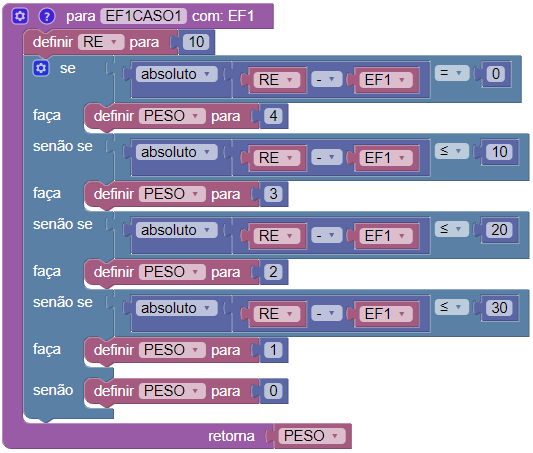
\includegraphics[width=0.9\linewidth]{chapters/appendixAnalytics/A02/C1EF1.png}  \end{tabular}
	} \\ \hline
	\multicolumn{3}{|c|}{\textbf{Python gerado}} \\ \hline
	\multicolumn{3}{|l|}{ \begin{tabular}[c]{@{}l@{}}import math \\ \# Nota Ponderada - EF1 - Caso 1 \\def EF1CASO1(EF1):\\ \quad global RE, PESO\\ \quad RE = 10\\ \quad if math.fabs(RE - EF1) == 0:\\ \quad \quad PESO = 4\\ \quad elif math.fabs(RE - EF1) <= 10: \\ \quad \quad PESO = 3\\ \quad elif math.fabs(RE - EF1) <= 20:\\ \quad \quad PESO = 2\\ \quad elif math.fabs(RE - EF1) <= 30:\\ \quad \quad PESO = 1\\ \quad else:\\ \quad \quad PESO = 0\\ \quad return PESO\end{tabular} }\\ \hline

	%EV1
	\multicolumn{3}{|c|}{\cellcolor[HTML]{DEDEDE}\textbf{Nota Ponderada - EV1}} \\ \hline
	\multicolumn{3}{|c|}{\textbf{Blocos}} \\ \hline
	\multicolumn{3}{|l|}{\begin{tabular}[c]{@{}l@{}} \\ 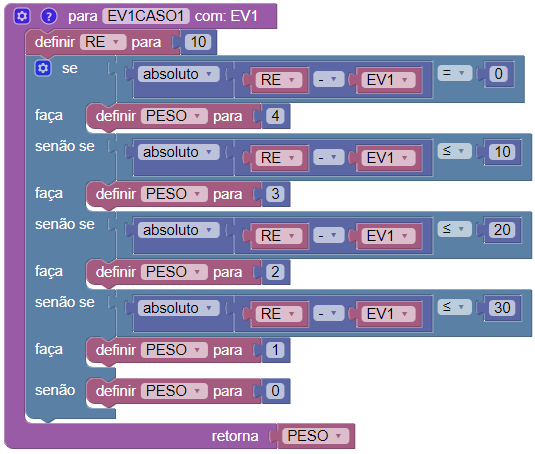
\includegraphics[width=0.9\linewidth]{chapters/appendixAnalytics/A02/C1EV1.png}  \end{tabular}
	} \\ \hline
	\multicolumn{3}{|c|}{\textbf{Python gerado}} \\ \hline
	\multicolumn{3}{|l|}{ \begin{tabular}[c]{@{}l@{}}import math \\ \# Nota Ponderada - EV1 - Caso 1\\ def EV1CASO1(EV1):\\ \quad global RE, PESO\\ \quad RE = 10\\ \quad if math.fabs(RE - EV1) == 0:\\ \quad \quad PESO = 4\\ \quad \quad elif math.fabs(RE - EV1) <= 10:\\ \quad \quad PESO = 3\\ \quad elif math.fabs(RE - EV1) <= 20:\\ \quad \quad PESO = 2\\ \quad elif math.fabs(RE - EV1) <= 30:\\ \quad \quad PESO = 1\\ \quad else:\\ \quad \quad PESO = 0\\ \quad return PESO \end{tabular} }\\ \hline

	%EV2
	\multicolumn{3}{|c|}{\cellcolor[HTML]{DEDEDE}\textbf{Nota Ponderada - EV2}} \\ \hline
	\multicolumn{3}{|c|}{\textbf{Blocos}} \\ \hline
	\multicolumn{3}{|l|}{\begin{tabular}[c]{@{}l@{}} \\ 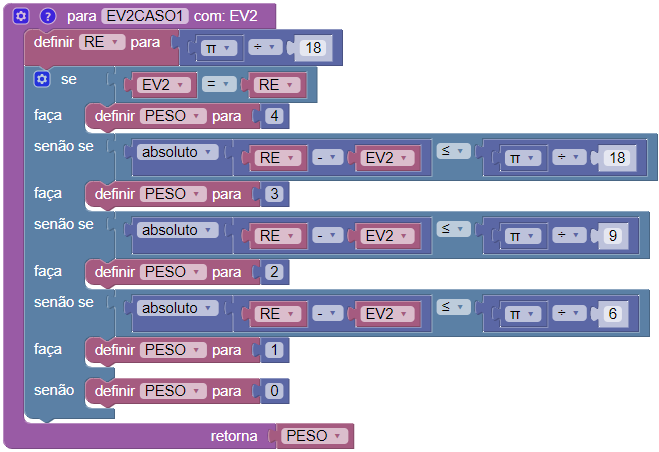
\includegraphics[width=0.9\linewidth]{chapters/appendixAnalytics/A02/C1EV2.png}  \end{tabular}
	} \\ \hline
	\multicolumn{3}{|c|}{\textbf{Python gerado}} \\ \hline
	\multicolumn{3}{|l|}{ \begin{tabular}[c]{@{}l@{}}import math\\ \# Nota Ponderada - EV2 - Caso 1\\def EV2CASO1(EV2):\\ \quad global RE, PESO\\ \quad RE = math.pi / 18\\ \quad if EV2 == RE:\\ \quad \quad PESO = 4\\ \quad elif math.fabs(RE - EV2) <= math.pi / 18:\\ \quad \quad PESO = 3\\ \quad elif math.fabs(RE - EV2) <= math.pi / 9:\\ \quad \quad PESO = 2\\ \quad elif math.fabs(RE - EV2) <= math.pi / 6:\\ \quad \quad PESO = 1\\ \quad else:\\ \quad \quad PESO = 0\\ \quad return PESO \end{tabular} }\\ \hline
	
\end{xltabular}

\pagebreak

%CASO 2
\begin{xltabular}{\textwidth}{|l|X|X|}
	\hline
	\endfirsthead
	
	\hline \multicolumn{3}{|c|}{continuação da página anterior} \\ \hline
	\endhead
	
	\hline \multicolumn{3}{|r|}{Continua na próxima página} \\ \hline
	\endfoot
	
	\hline
	\endlastfoot
	
	\multicolumn{3}{|c|}{\cellcolor[HTML]{C0C0C0}\textbf{CASO DE TESTE 2}} \\ \hline
	
	%EF1
	\multicolumn{3}{|c|}{\cellcolor[HTML]{DEDEDE}\textbf{Nota Ponderada - EF1}} \\ \hline
	\multicolumn{3}{|c|}{\textbf{Blocos}} \\ \hline
	\multicolumn{3}{|l|}{\begin{tabular}[c]{@{}l@{}} \\ 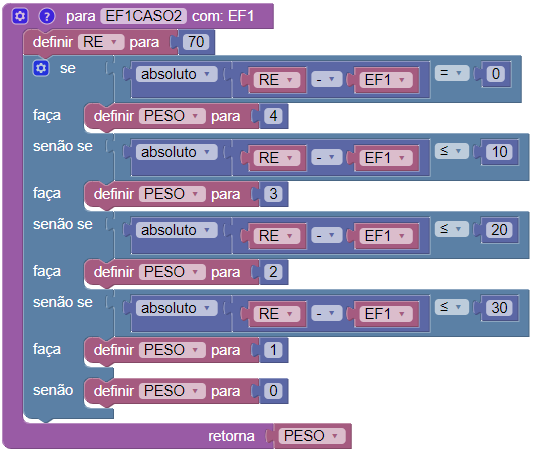
\includegraphics[width=0.9\linewidth]{chapters/appendixAnalytics/A02/C2EF1.png}  \end{tabular}
	} \\ \hline
	\multicolumn{3}{|c|}{\textbf{Python gerado}} \\ \hline
	\multicolumn{3}{|l|}{ \begin{tabular}[c]{@{}l@{}}import math \\ \# Nota Ponderada - EF1 - Caso 2\\ def EF1CASO2(EF1):\\ \quad global RE, PESO\\ \quad RE = 70\\ \quad if math.fabs(RE - EF1) == 0:\\ \quad \quad PESO = 4\\ \quad elif math.fabs(RE - EF1) <= 10:\\ \quad \quad PESO = 3\\ \quad elif math.fabs(RE - EF1) <= 20:\\ \quad \quad PESO = 2\\ \quad elif math.fabs(RE - EF1) <= 30:\\ \quad \quad PESO = 1\\ \quad else:\\ \quad \quad PESO = 0\\ \quad return PESO \end{tabular} }\\ \hline
	
	%EV1
	\multicolumn{3}{|c|}{\cellcolor[HTML]{DEDEDE}\textbf{Nota Ponderada - EV1}} \\ \hline
	\multicolumn{3}{|c|}{\textbf{Blocos}} \\ \hline
	\multicolumn{3}{|l|}{\begin{tabular}[c]{@{}l@{}} \\ 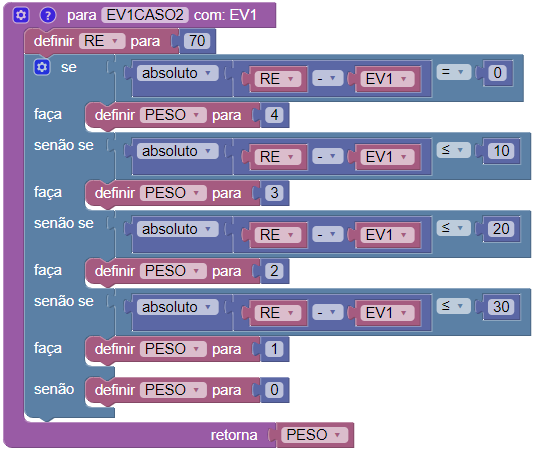
\includegraphics[width=0.9\linewidth]{chapters/appendixAnalytics/A02/C2EV1.png}  \end{tabular}
	} \\ \hline
	\multicolumn{3}{|c|}{\textbf{Python gerado}} \\ \hline
	\multicolumn{3}{|l|}{ \begin{tabular}[c]{@{}l@{}}import math \\ \# Nota Ponderada - EV1 - Caso 2\\ def EV1CASO2(EV1):\\ \quad global RE, PESO\\ \quad RE = 70\\ \quad if math.fabs(RE - EV1) == 0:\\ \quad \quad PESO = 4\\ \quad elif math.fabs(RE - EV1) <= 10:\\ \quad \quad PESO = 3\\ \quad elif math.fabs(RE - EV1) <= 20:\\ \quad \quad PESO = 2\\ \quad elif math.fabs(RE - EV1) <= 30:\\ \quad \quad PESO = 1\\ \quad else:\\ \quad \quad PESO = 0\\ \quad return PESO \end{tabular} }\\ \hline
	
	%EV2
	\multicolumn{3}{|c|}{\cellcolor[HTML]{DEDEDE}\textbf{Nota Ponderada - EV2}} \\ \hline
	\multicolumn{3}{|c|}{\textbf{Blocos}} \\ \hline
	\multicolumn{3}{|l|}{\begin{tabular}[c]{@{}l@{}} \\ 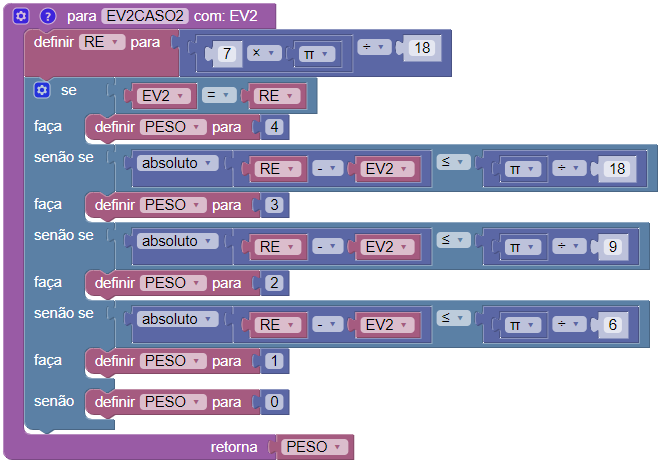
\includegraphics[width=0.9\linewidth]{chapters/appendixAnalytics/A02/C2EV2.png}  \end{tabular}
	} \\ \hline
	\multicolumn{3}{|c|}{\textbf{Python gerado}} \\ \hline
	\multicolumn{3}{|l|}{ \begin{tabular}[c]{@{}l@{}}import math\\ \# Nota Ponderada - EV2 - Caso 2\\ def EV2CASO2(EV2): \\ \quad global RE, PESO \\ \quad RE = (7 * math.pi) / 18\\ \quad if EV2 == RE:\\ \qquad PESO = 4\\ \quad elif math.fabs(RE - EV2) <= math.pi / 18:\\ \qquad PESO = 3\\ \quad elif math.fabs(RE - EV2) <= math.pi / 9:\\\qquad PESO = 2\\ \quad elif math.fabs(RE - EV2) <= math.pi / 6:\\ \qquad PESO = 1\\ \quad else:\\ \qquad PESO = 0\\ \quad return PESO \end{tabular} }\\ \hline
	
\end{xltabular}

\pagebreak
%CASO 3
\begin{xltabular}{\textwidth}{|l|X|X|}
	\hline
	\endfirsthead
	
	\hline \multicolumn{3}{|c|}{continuação da página anterior} \\ \hline
	\endhead
	
	\hline \multicolumn{3}{|r|}{Continua na próxima página} \\ \hline
	\endfoot
	
	\hline
	\endlastfoot
	
	\multicolumn{3}{|c|}{\cellcolor[HTML]{C0C0C0}\textbf{CASO DE TESTE 3}} \\ \hline
	
	%EF1
	\multicolumn{3}{|c|}{\cellcolor[HTML]{DEDEDE}\textbf{Nota Ponderada - EF1}} \\ \hline
	\multicolumn{3}{|c|}{\textbf{Blocos}} \\ \hline
	\multicolumn{3}{|l|}{\begin{tabular}[c]{@{}l@{}} \\ 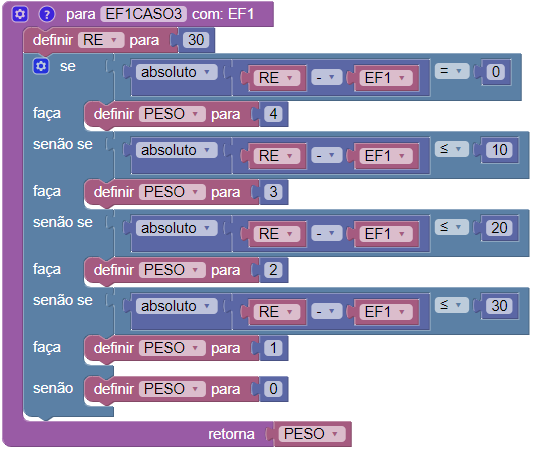
\includegraphics[width=0.9\linewidth]{chapters/appendixAnalytics/A02/C3EF1.png}  \end{tabular}
	} \\ \hline
	\multicolumn{3}{|c|}{\textbf{Python gerado}} \\ \hline
	\multicolumn{3}{|l|}{ \begin{tabular}[c]{@{}l@{}}import math \\ \# Nota Ponderada - EF1 - Caso 3\\ def EF1CASO3(EF1):\\ \quad global RE, PESO\\ \quad RE = 30 \\ \quad if math.fabs(RE - EF1) == 0:\\ \qquad PESO = 4\\ \quad elif math.fabs(RE - EF1) <= 10: \\ \qquad PESO = 3\\ \quad elif math.fabs(RE - EF1) <= 20:\\ \qquad PESO = 2\\ \quad elif math.fabs(RE - EF1) <= 30:\\ \qquad PESO = 1\\ \quad else:\\ \qquad PESO = 0\\ \quad return PESO \end{tabular} }\\ \hline
	
	%EV1
	\multicolumn{3}{|c|}{\cellcolor[HTML]{DEDEDE}\textbf{Nota Ponderada - EV1}} \\ \hline
	\multicolumn{3}{|c|}{\textbf{Blocos}} \\ \hline
	\multicolumn{3}{|l|}{\begin{tabular}[c]{@{}l@{}} \\ 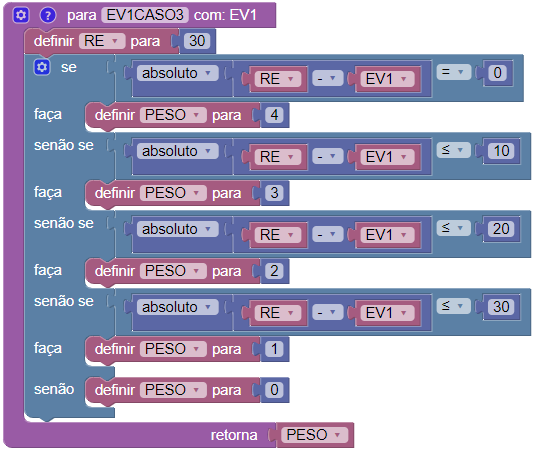
\includegraphics[width=0.9\linewidth]{chapters/appendixAnalytics/A02/C3EV1.png}  \end{tabular}
	} \\ \hline
	\multicolumn{3}{|c|}{\textbf{Python gerado}} \\ \hline
	\multicolumn{3}{|l|}{ \begin{tabular}[c]{@{}l@{}}import math \\ \# Nota Ponderada - EV1 - Caso 3\\ def EV1CASO3(EV1):\\ \quad global RE, PESO\\ \quad RE = 30\\ \quad if math.fabs(RE - EV1) == 0:\\ \qquad PESO = 4\\ \quad elif math.fabs(RE - EV1) <= 10:\\ \qquad PESO = 3\\ \quad elif math.fabs(RE - EV1) <= 20:\\ \qquad PESO = 2\\ \quad elif math.fabs(RE - EV1) <= 30:\\ \qquad PESO = 1\\ \quad else:\\ \qquad PESO = 0\\ \quad return PESO \end{tabular} }\\ \hline

	%EV2
	\multicolumn{3}{|c|}{\cellcolor[HTML]{DEDEDE}\textbf{Nota Ponderada - EV2}} \\ \hline
	\multicolumn{3}{|c|}{\textbf{Blocos}} \\ \hline
	\multicolumn{3}{|l|}{\begin{tabular}[c]{@{}l@{}} \\ 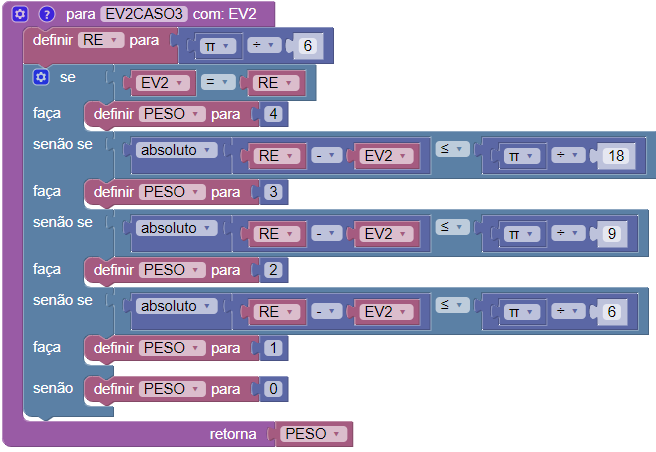
\includegraphics[width=0.9\linewidth]{chapters/appendixAnalytics/A02/C3EV2.png}  \end{tabular}
	} \\ \hline
	\multicolumn{3}{|c|}{\textbf{Python gerado}} \\ \hline
	\multicolumn{3}{|l|}{ \begin{tabular}[c]{@{}l@{}}import math\\ \# Nota Ponderada - EV2 - Caso 3\\ def EV2CASO3(EV2):\\ \quad global RE, PESO\\ \quad RE = math.pi / 6\\ \quad if EV2 == RE:\\ \qquad PESO = 4\\ \quad elif math.fabs(RE - EV2) <= math.pi / 18:\\ \qquad PESO = 3\\ \quad elif math.fabs(RE - EV2) <= math.pi / 9:\\ \qquad PESO = 2\\ \quad elif math.fabs(RE - EV2) <= math.pi / 6:\\ \qquad PESO = 1\\ \quad else:\\ \qquad PESO = 0\\ \quad return PESO \end{tabular} }\\ \hline

\end{xltabular}

\pagebreak
%CASO 4
\begin{xltabular}{\textwidth}{|l|X|X|}
	\hline
	\endfirsthead
	
	\hline \multicolumn{3}{|c|}{continuação da página anterior} \\ \hline
	\endhead
	
	\hline \multicolumn{3}{|r|}{Continua na próxima página} \\ \hline
	\endfoot
	
	\hline
	\endlastfoot
	
	\multicolumn{3}{|c|}{\cellcolor[HTML]{C0C0C0}\textbf{CASO DE TESTE 4}} \\ \hline
	
	%EF1
	\multicolumn{3}{|c|}{\cellcolor[HTML]{DEDEDE}\textbf{Nota Ponderada - EF1}} \\ \hline
	\multicolumn{3}{|c|}{\textbf{Blocos}} \\ \hline
	\multicolumn{3}{|l|}{\begin{tabular}[c]{@{}l@{}} \\ 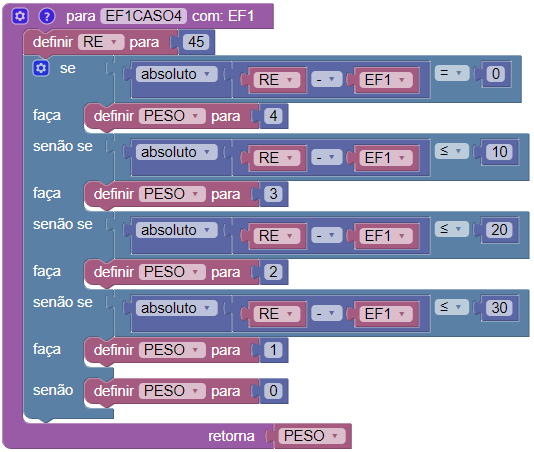
\includegraphics[width=0.9\linewidth]{chapters/appendixAnalytics/A02/C4EF1.png}  \end{tabular}
	} \\ \hline
	\multicolumn{3}{|c|}{\textbf{Python gerado}} \\ \hline
	\multicolumn{3}{|l|}{ \begin{tabular}[c]{@{}l@{}}import math \\ \# Nota Ponderada - EF1 - Caso 4\\ def EF1CASO4(EF1):\\ \quad global RE, PESO\\ \quad RE = 45\\ \quad if math.fabs(RE - EF1) == 0:\\ \qquad PESO = 4\\ \quad elif math.fabs(RE - EF1) <= 10:\\ \qquad PESO = 3\\ \quad elif math.fabs(RE - EF1) <= 20:\\ \qquad PESO = 2\\ \quad elif math.fabs(RE - EF1) <= 30:\\ \qquad PESO = 1\\ \quad else: \\ \qquad PESO = 0\\ \quad return PESO \end{tabular} }\\ \hline
	
	%EV1
	\multicolumn{3}{|c|}{\cellcolor[HTML]{DEDEDE}\textbf{Nota Ponderada - EV1}} \\ \hline
	\multicolumn{3}{|c|}{\textbf{Blocos}} \\ \hline
	\multicolumn{3}{|l|}{\begin{tabular}[c]{@{}l@{}} \\ 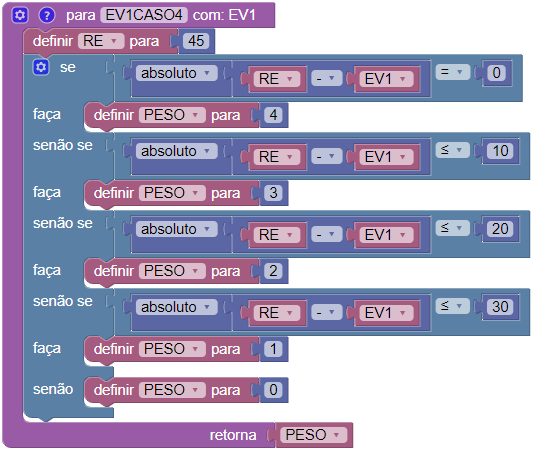
\includegraphics[width=0.9\linewidth]{chapters/appendixAnalytics/A02/C4EV1.png}  \end{tabular}
	} \\ \hline
	\multicolumn{3}{|c|}{\textbf{Python gerado}} \\ \hline
	\multicolumn{3}{|l|}{ \begin{tabular}[c]{@{}l@{}}import math \\ \# Nota Ponderada - EV1 - Caso 4\\ def EV1CASO4(EV1):\\ \quad global RE, PESO\\ \quad RE = 45\\ \quad if math.fabs(RE - EV1) == 0:\\ \qquad PESO = 4\\ \quad elif math.fabs(RE - EV1) <= 10:\\ \qquad PESO = 3\\ \quad elif math.fabs(RE - EV1) <= 20:\\ \qquad PESO = 2\\ \quad elif math.fabs(RE - EV1) <= 30:\\ \qquad PESO = 1\\ \quad else:\\ \qquad PESO = 0\\ \quad return PESO \end{tabular} }\\ \hline
	
	%EV2
	\multicolumn{3}{|c|}{\cellcolor[HTML]{DEDEDE}\textbf{Nota Ponderada - EV2}} \\ \hline
	\multicolumn{3}{|c|}{\textbf{Blocos}} \\ \hline
	\multicolumn{3}{|l|}{\begin{tabular}[c]{@{}l@{}} \\ 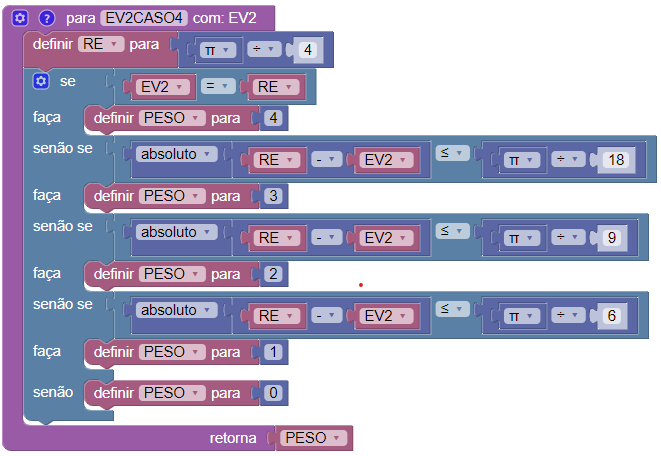
\includegraphics[width=0.9\linewidth]{chapters/appendixAnalytics/A02/C4EV2.png}  \end{tabular}
	} \\ \hline
	\multicolumn{3}{|c|}{\textbf{Python gerado}} \\ \hline
	\multicolumn{3}{|l|}{ \begin{tabular}[c]{@{}l@{}}import math \\ \# Nota Ponderada - EV2 - Caso 4\\ \quad def EV2CASO4(EV2):\\ \quad global RE, PESO\\ \qquad RE = math.pi / 4\\ \quad if EV2 == RE:\\ \qquad PESO = 4\\ \quad elif math.fabs(RE - EV2) <= math.pi / 18:\\ \qquad PESO = 3\\ \quad elif math.fabs(RE - EV2) <= math.pi / 9:\\ \qquad PESO = 2\\ \quad elif math.fabs(RE - EV2) <= math.pi / 6:\\ \qquad PESO = 1\\ \quad else:\\ \qquad PESO = 0\\ \quad return PESO \end{tabular} }\\ \hline
	
\end{xltabular}

\pagebreak
%CASO 5
\begin{xltabular}{\textwidth}{|l|X|X|}
	\hline
	\endfirsthead
	
	\hline \multicolumn{3}{|c|}{continuação da página anterior} \\ \hline
	\endhead
	
	\hline \multicolumn{3}{|r|}{Continua na próxima página} \\ \hline
	\endfoot
	
	\hline
	\endlastfoot
	
	\multicolumn{3}{|c|}{\cellcolor[HTML]{C0C0C0}\textbf{CASO DE TESTE 5}} \\ \hline
	
	%EF1
	\multicolumn{3}{|c|}{\cellcolor[HTML]{DEDEDE}\textbf{Nota Ponderada - EF1}} \\ \hline
	\multicolumn{3}{|c|}{\textbf{Blocos}} \\ \hline
	\multicolumn{3}{|l|}{\begin{tabular}[c]{@{}l@{}} \\ 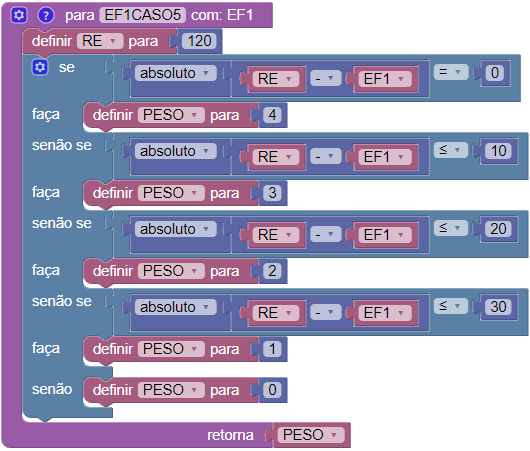
\includegraphics[width=0.9\linewidth]{chapters/appendixAnalytics/A02/C5EF1.png}  \end{tabular}
	} \\ \hline
	\multicolumn{3}{|c|}{\textbf{Python gerado}} \\ \hline
	\multicolumn{3}{|l|}{ \begin{tabular}[c]{@{}l@{}}import math \\ \# Nota Ponderada - EF1 - Caso 5\\ def EF1CASO5(EF1):\\ \quad global RE, PESO\\ \quad RE = 120\\ \quad if math.fabs(RE - EF1) == 0:\\ \qquad PESO = 4\\ \quad elif math.fabs(RE - EF1) <= 10:\\ \qquad PESO = 3\\ \quad elif math.fabs(RE - EF1) <= 20:\\ \qquad PESO = 2\\ \quad elif math.fabs(RE - EF1) <= 30:\\ \qquad PESO = 1\\ \quad else:\\ \qquad PESO = 0\\ \quad return PESO \end{tabular} }\\ \hline
	
	%EV1
	\multicolumn{3}{|c|}{\cellcolor[HTML]{DEDEDE}\textbf{Nota Ponderada - EV1}} \\ \hline
	\multicolumn{3}{|c|}{\textbf{Blocos}} \\ \hline
	\multicolumn{3}{|l|}{\begin{tabular}[c]{@{}l@{}} \\ 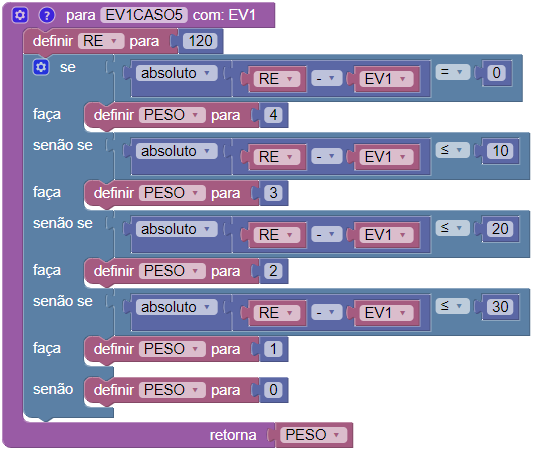
\includegraphics[width=0.9\linewidth]{chapters/appendixAnalytics/A02/C5EV1.png}  \end{tabular}
	} \\ \hline
	\multicolumn{3}{|c|}{\textbf{Python gerado}} \\ \hline
	\multicolumn{3}{|l|}{ \begin{tabular}[c]{@{}l@{}}import math \\ \# Nota Ponderada - EV1 - Caso 5\\ def EV1CASO5(EV1):\\ \quad global RE, PESO\\ \quad RE = 120\\ \quad if math.fabs(RE - EV1) == 0:\\ \qquad PESO = 4\\ \quad elif math.fabs(RE - EV1) <= 10:\\ \qquad PESO = 3\\ \quad elif math.fabs(RE - EV1) <= 20:\\ \qquad PESO = 2\\ \quad elif math.fabs(RE - EV1) <= 30:\\ \qquad PESO = 1\\ \quad else:\\ \qquad PESO = 0\\ \quad return PESO \end{tabular} }\\ \hline
	
	%EV2
	\multicolumn{3}{|c|}{\cellcolor[HTML]{DEDEDE}\textbf{Nota Ponderada - EV2}} \\ \hline
	\multicolumn{3}{|c|}{\textbf{Blocos}} \\ \hline
	\multicolumn{3}{|l|}{\begin{tabular}[c]{@{}l@{}} \\ 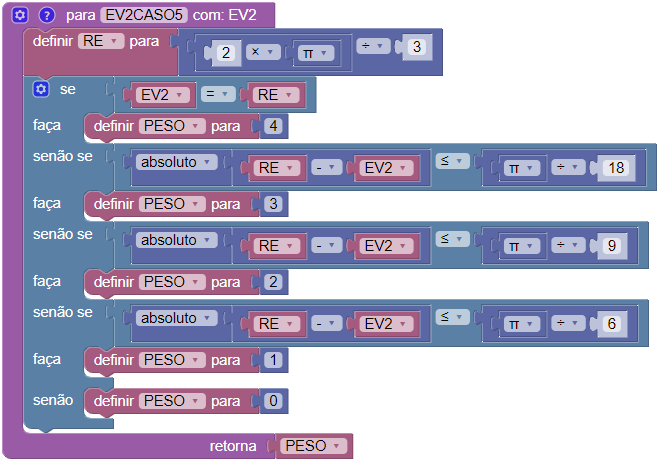
\includegraphics[width=0.9\linewidth]{chapters/appendixAnalytics/A02/C5EV2.png}  \end{tabular}
	} \\ \hline
	\multicolumn{3}{|c|}{\textbf{Python gerado}} \\ \hline
	\multicolumn{3}{|l|}{ \begin{tabular}[c]{@{}l@{}}import math\\ \# Nota Ponderada - EV2 - Caso 5\\ def EV2CASO5(EV2):\\ \quad	global RE, PESO\\ \quad RE = (2 * math.pi) / 3\\ \quad if EV2 == RE:\\ \qquad PESO = 4\\ \quad elif math.fabs(RE - EV2) <= math.pi / 18:\\ \qquad PESO = 3\\ \quad elif math.fabs(RE - EV2) <= math.pi / 9:\\ \qquad PESO = 2\\ \quad elif math.fabs(RE - EV2) <= math.pi / 6:\\ \qquad PESO = 1\\ \quad else:\\ \qquad PESO = 0\\ \quad return PESO \end{tabular} }\\ \hline
	
\end{xltabular}

\pagebreak
%CASO 6
\begin{xltabular}{\textwidth}{|l|X|X|}
	\hline
	\endfirsthead
	
	\hline \multicolumn{3}{|c|}{continuação da página anterior} \\ \hline
	\endhead
	
	\hline \multicolumn{3}{|r|}{Continua na próxima página} \\ \hline
	\endfoot
	
	\hline
	\endlastfoot
	
	\multicolumn{3}{|c|}{\cellcolor[HTML]{C0C0C0}\textbf{CASO DE TESTE 6}} \\ \hline
	
	%EF1
	\multicolumn{3}{|c|}{\cellcolor[HTML]{DEDEDE}\textbf{Nota Ponderada - EF1}} \\ \hline
	\multicolumn{3}{|c|}{\textbf{Blocos}} \\ \hline
	\multicolumn{3}{|l|}{\begin{tabular}[c]{@{}l@{}} \\ 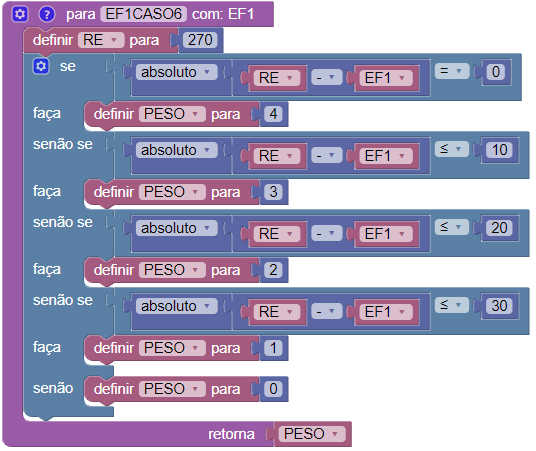
\includegraphics[width=0.9\linewidth]{chapters/appendixAnalytics/CASO6NPEF1.png}  \end{tabular}
	} \\ \hline
	\multicolumn{3}{|c|}{\textbf{Python gerado}} \\ \hline
	\multicolumn{3}{|l|}{ \begin{tabular}[c]{@{}l@{}}import math \\ \# Nota Ponderada - Caso 6\\ def EF1CASO6(EF1):\\ \quad global RE, PESO\\ \quad RE = 270\\ \quad	if math.fabs(RE - EF1) == 0:\\	\quad \quad PESO = 4\\ \quad elif math.fabs(RE - EF1) <= 10:\\ \quad \quad PESO = 3\\	\quad elif math.fabs(RE - EF1) <= 20:\\ \quad \quad	PESO = 2\\ \quad elif math.fabs(RE - EF1) <= 30:\\ \quad \quad PESO = 1\\ \quad	else:\\ \quad \quad	PESO = 0\\ \quad return PESO \end{tabular} }\\ \hline
	
	%EV1
	\multicolumn{3}{|c|}{\cellcolor[HTML]{DEDEDE}\textbf{Nota Ponderada - EV1}} \\ \hline
	\multicolumn{3}{|c|}{\textbf{Blocos}} \\ \hline
	\multicolumn{3}{|l|}{\begin{tabular}[c]{@{}l@{}} \\ 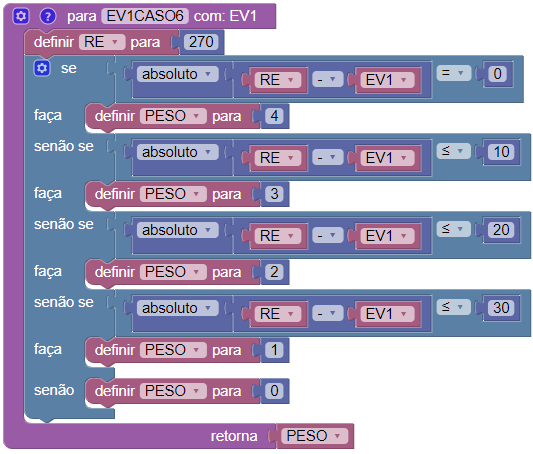
\includegraphics[width=0.9\linewidth]{chapters/appendixAnalytics/CASO6NPEV1.png}  \end{tabular}
	} \\ \hline
	\multicolumn{3}{|c|}{\textbf{Python gerado}} \\ \hline
	\multicolumn{3}{|l|}{ \begin{tabular}[c]{@{}l@{}}import math \\ \# Nota Ponderada - Caso 6\\ def EV1CASO6(EV1):\\ \quad global RE, PESO\\ \quad RE = 270\\ \quad	if math.fabs(RE - EV1) == 0:\\	\quad \quad PESO = 4\\ \quad elif math.fabs(RE - EV1) <= 10:\\ \quad \quad PESO = 3\\	\quad elif math.fabs(RE - EV1) <= 20:\\ \quad \quad	PESO = 2\\ \quad elif math.fabs(RE - EV1) <= 30:\\ \quad \quad PESO = 1\\ \quad	else:\\ \quad \quad	PESO = 0\\ \quad return PESO \end{tabular} }\\ \hline
	
	%EV2
	\multicolumn{3}{|c|}{\cellcolor[HTML]{DEDEDE}\textbf{Nota Ponderada - EV2}} \\ \hline
	\multicolumn{3}{|c|}{\textbf{Blocos}} \\ \hline
	\multicolumn{3}{|l|}{\begin{tabular}[c]{@{}l@{}} \\ 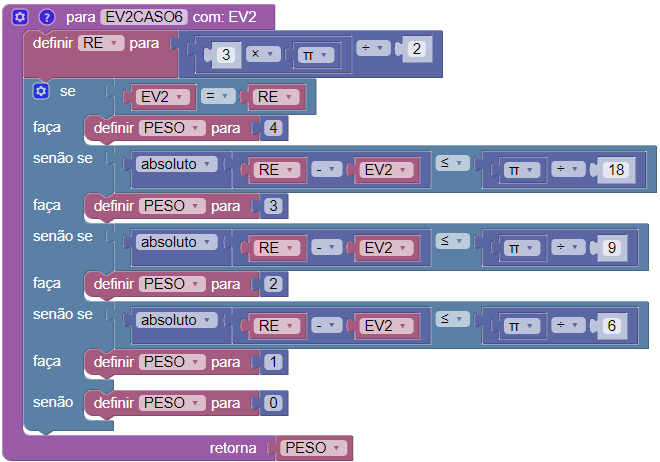
\includegraphics[width=0.9\linewidth]{chapters/appendixAnalytics/CASO6NPEV2.png}  \end{tabular}
	} \\ \hline
	\multicolumn{3}{|c|}{\textbf{Python gerado}} \\ \hline
	\multicolumn{3}{|l|}{ \begin{tabular}[c]{@{}l@{}}import math \\ \# Nota Ponderada - EV2 - Caso 6\\ def EV2CASO6(EV2):\\ \quad global RE, PESO \\ \quad RE = (3 * math.pi) / 2 \\ \quad if EV2 == RE:\\ \quad \quad	PESO = 4\\ \quad	elif math.fabs(RE - EV2) <= math.pi / 18:\\ \quad \quad PESO = 3\\ \quad	elif math.fabs(RE - EV2) <= math.pi / 9:\\ \quad \quad	PESO = 2\\ \quad	elif math.fabs(RE - EV2) <= math.pi / 6:\\ \quad \quad PESO = 1\\ \quad	else: \\ \quad \quad	PESO = 0\\ \quad return PESO \end{tabular} }\\ \hline
	
\end{xltabular}

\pagebreak
%CASO 7
\begin{xltabular}{\textwidth}{|l|X|X|}
	\hline
	\endfirsthead
	
	\hline \multicolumn{3}{|c|}{continuação da página anterior} \\ \hline
	\endhead
	
	\hline \multicolumn{3}{|r|}{Continua na próxima página} \\ \hline
	\endfoot
	
	\hline
	\endlastfoot
	
	\multicolumn{3}{|c|}{\cellcolor[HTML]{C0C0C0}\textbf{CASO DE TESTE 7}} \\ \hline
	
	%EF1
	\multicolumn{3}{|c|}{\cellcolor[HTML]{DEDEDE}\textbf{Nota Ponderada - EF1}} \\ \hline
	\multicolumn{3}{|c|}{\textbf{Blocos}} \\ \hline
	\multicolumn{3}{|l|}{\begin{tabular}[c]{@{}l@{}} \\ 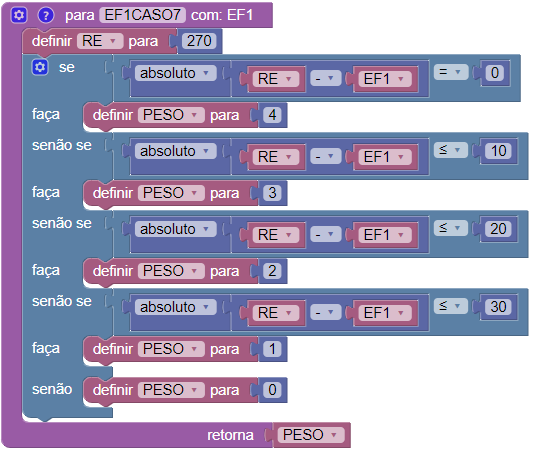
\includegraphics[width=0.9\linewidth]{chapters/appendixAnalytics/CASO7NPEF1.png}  \end{tabular}
	} \\ \hline
	\multicolumn{3}{|c|}{\textbf{Python gerado}} \\ \hline
	\multicolumn{3}{|l|}{ \begin{tabular}[c]{@{}l@{}}import math\\ \# Nota Ponderada - EF1 - Caso 7\\ def EF1CASO7(EF1):\\ \quad global RE, PESO\\ \quad  RE = 270\\ \quad if math.fabs(RE - EF1) == 0:\\ \quad \quad PESO = 4\\ \quad elif math.fabs(RE - EF1) <= 10:\\ \quad \quad PESO = 3\\ \quad elif math.fabs(RE - EF1) <= 20:\\ \quad \quad PESO = 2\\ \quad elif math.fabs(RE - EF1) <= 30:\\ \quad \quad PESO = 1\\ \quad else:\\ \quad \quad PESO = 0\\ \quad return PESO \end{tabular} }\\ \hline
	
	%EV1
	\multicolumn{3}{|c|}{\cellcolor[HTML]{DEDEDE}\textbf{Nota Ponderada - EV1}} \\ \hline
	\multicolumn{3}{|c|}{\textbf{Blocos}} \\ \hline
	\multicolumn{3}{|l|}{\begin{tabular}[c]{@{}l@{}} \\ 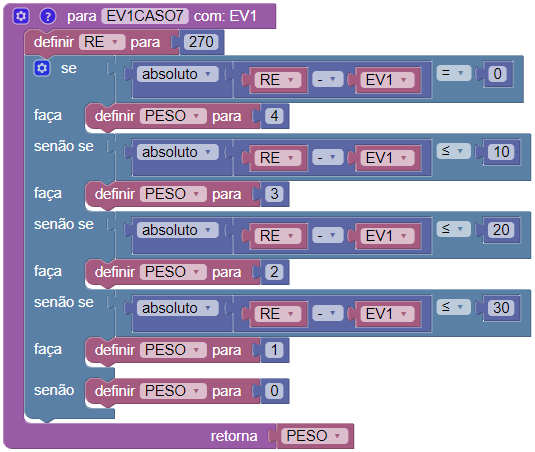
\includegraphics[width=0.9\linewidth]{chapters/appendixAnalytics/CASO7NPEV1.png}  \end{tabular}
	} \\ \hline
	\multicolumn{3}{|c|}{\textbf{Python gerado}} \\ \hline
	\multicolumn{3}{|l|}{ \begin{tabular}[c]{@{}l@{}}import math \\ \# Nota Ponderada - EV1 - Caso 7\\ def EV1CASO7(EV1):\\ \quad global RE, PESO\\ \quad RE = 270\\ \quad if math.fabs(RE - EV1) == 0:\\ \quad \quad PESO = 4\\ \quad elif math.fabs(RE - EV1) <= 10:\\ \quad \quad PESO = 3\\ \quad elif math.fabs(RE - EV1) <= 20:\\ \quad \quad PESO = 2\\ \quad elif math.fabs(RE - EV1) <= 30:\\ \quad \quad PESO = 1\\ \quad else:\\ \quad \quad PESO = 0\\ \quad return PESO \end{tabular} }\\ \hline
	
	%EV2
	\multicolumn{3}{|c|}{\cellcolor[HTML]{DEDEDE}\textbf{Nota Ponderada - EV2}} \\ \hline
	\multicolumn{3}{|c|}{\textbf{Blocos}} \\ \hline
	\multicolumn{3}{|l|}{\begin{tabular}[c]{@{}l@{}} \\ 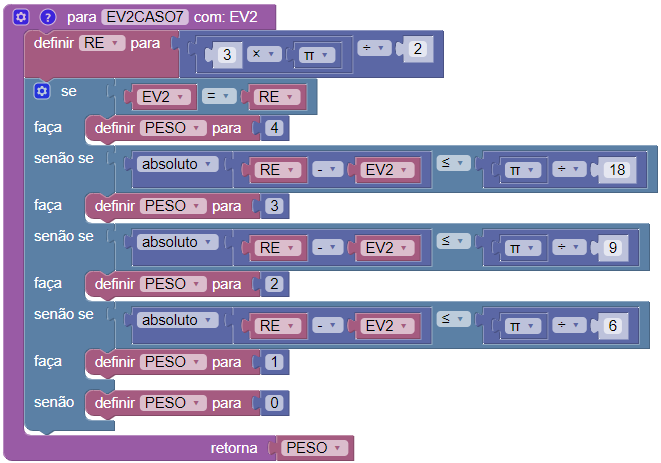
\includegraphics[width=0.9\linewidth]{chapters/appendixAnalytics/CASO7NPEV2.png}  \end{tabular}
	} \\ \hline
	\multicolumn{3}{|c|}{\textbf{Python gerado}} \\ \hline
	\multicolumn{3}{|l|}{ \begin{tabular}[c]{@{}l@{}}import math \\ \# Nota Ponderada - EV2 - Caso 7\\ def EV2CASO7(EV2):\\ \quad global RE, PESO\\ \quad RE = (3 * math.pi) / 2\\ \quad if EV2 == RE:\\ \quad \quad PESO = 4\\ \quad elif math.fabs(RE - EV2) <= math.pi / 18:\\ \quad \quad PESO = 3\\ \quad elif math.fabs(RE - EV2) <= math.pi / 9:\\ \quad \quad PESO = 2\\ \quad elif math.fabs(RE - EV2) <= math.pi / 6: \\ \quad \quad PESO = 1\\ \quad else:\\ \quad \quad PESO = 0\\ \quad return PESO \end{tabular} }\\ \hline
	
\end{xltabular}

\pagebreak
%CASO 8
\begin{xltabular}{\textwidth}{|l|X|X|}
	\hline
	\endfirsthead
	
	\hline \multicolumn{3}{|c|}{continuação da página anterior} \\ \hline
	\endhead
	
	\hline \multicolumn{3}{|r|}{Continua na próxima página} \\ \hline
	\endfoot
	
	\hline
	\endlastfoot
	
	\multicolumn{3}{|c|}{\cellcolor[HTML]{C0C0C0}\textbf{CASO DE TESTE 8}} \\ \hline
	
	%EF1
	\multicolumn{3}{|c|}{\cellcolor[HTML]{DEDEDE}\textbf{Nota Ponderada - EF1}} \\ \hline
	\multicolumn{3}{|c|}{\textbf{Blocos}} \\ \hline
	\multicolumn{3}{|l|}{\begin{tabular}[c]{@{}l@{}} \\ 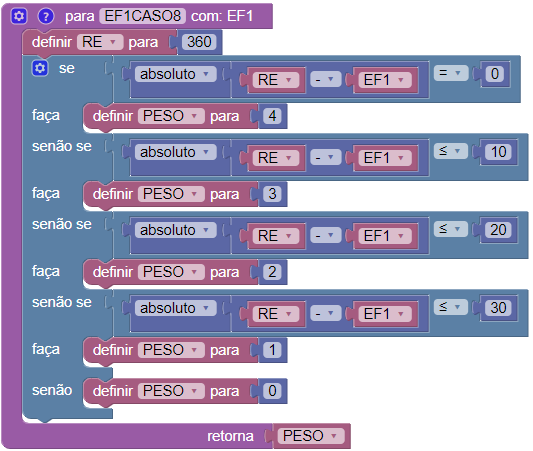
\includegraphics[width=0.9\linewidth]{chapters/appendixAnalytics/CASO8NPEF1.png}  \end{tabular}
	} \\ \hline
	\multicolumn{3}{|c|}{\textbf{Python gerado}} \\ \hline
	\multicolumn{3}{|l|}{ \begin{tabular}[c]{@{}l@{}}import math\\ \# Nota Ponderada - EF1 - Caso 8\\ def EF1CASO8(EF1):\\ \quad global RE, PESO\\ \quad RE = 360\\ \quad if math.fabs(RE - EF1) == 0:\\ \quad \quad PESO = 4\\ \quad elif math.fabs(RE - EF1) <= 10:\\ \quad \quad PESO = 3\\ \quad elif math.fabs(RE - EF1) <= 20:\\ \quad \quad PESO = 2\\ \quad elif math.fabs(RE - EF1) <= 30:\\ \quad \quad PESO = 1\\ \quad else:\\ \quad \quad PESO = 0\\ \quad return PESO \end{tabular} }\\ \hline
	
	%EV1
	\multicolumn{3}{|c|}{\cellcolor[HTML]{DEDEDE}\textbf{Nota Ponderada - EV1}} \\ \hline
	\multicolumn{3}{|c|}{\textbf{Blocos}} \\ \hline
	\multicolumn{3}{|l|}{\begin{tabular}[c]{@{}l@{}} \\ 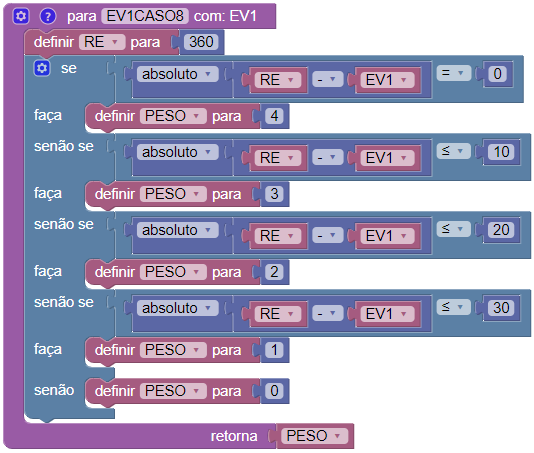
\includegraphics[width=0.9\linewidth]{chapters/appendixAnalytics/CASO8NPEV1.png}  \end{tabular}
	} \\ \hline
	\multicolumn{3}{|c|}{\textbf{Python gerado}} \\ \hline
	\multicolumn{3}{|l|}{ \begin{tabular}[c]{@{}l@{}}import math \\ \# Nota Ponderada - EV1 - Caso 8\\ def EV1CASO8(EV1):\\ \quad global RE, PESO\\ \quad RE = 360\\ \quad if math.fabs(RE - EV1) == 0:\\ \quad \quad PESO = 4\\ \quad elif math.fabs(RE - EV1) <= 10:\\ \quad \quad PESO = 3\\ \quad elif math.fabs(RE - EV1) <= 20:\\ \quad \quad PESO = 2\\ \quad elif math.fabs(RE - EV1) <= 30:\\ \quad \quad PESO = 1\\ \quad else:\\ \quad \quad PESO = 0\\ \quad return PESO \end{tabular} }\\ \hline
	
	%EV2
	\multicolumn{3}{|c|}{\cellcolor[HTML]{DEDEDE}\textbf{Nota Ponderada - EV2}} \\ \hline
	\multicolumn{3}{|c|}{\textbf{Blocos}} \\ \hline
	\multicolumn{3}{|l|}{\begin{tabular}[c]{@{}l@{}} \\ 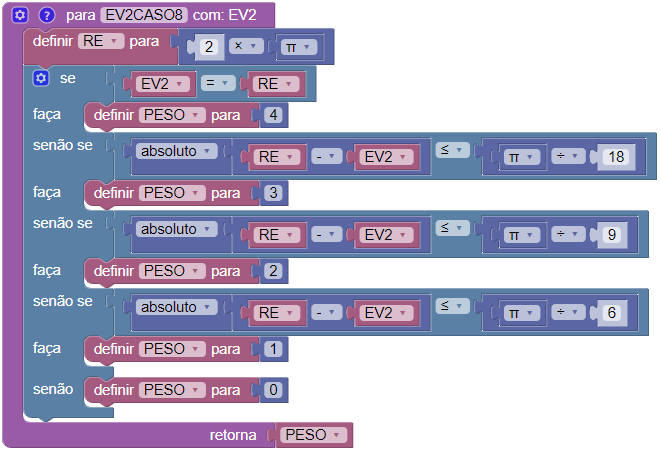
\includegraphics[width=0.9\linewidth]{chapters/appendixAnalytics/CASO8NPEV2.png}  \end{tabular}
	} \\ \hline
	\multicolumn{3}{|c|}{\textbf{Python gerado}} \\ \hline
	\multicolumn{3}{|l|}{ \begin{tabular}[c]{@{}l@{}}import math \\ \# Nota Ponderada - EV2 - Caso 8\\ def EV2CASO8(EV2):\\ \quad global RE, PESO\\ \quad RE = 2 * math.pi\\ \quad if EV2 == RE:\\ \quad \quad PESO = 4\\ \quad elif math.fabs(RE - EV2) <= math.pi / 18:\\ \quad \quad PESO = 3\\ \quad elif math.fabs(RE - EV2) <= math.pi / 9:\\ \quad \quad PESO = 2\\ \quad elif math.fabs(RE - EV2) <= math.pi / 6:\\ \quad \quad PESO = 1\\ \quad else:\\ \quad \quad PESO = 0\\ \quad return PESO \end{tabular} }\\ \hline
	
\end{xltabular}

%%CASO 1
%\begin{table}[htb!]
%	\caption{Nota Ponderada - Caso de Teste 1 - EF1}
%	\centering
%	\begin{tabular}{|c|c|}
%		\hline
%		\multicolumn{2}{|c|}{\cellcolor[HTML]{DEDEDE}\textbf{NP - CASO 1 - EF1}} \\ \hline
%		\textbf{Blocos} & \multicolumn{1}{c|}{\textbf{Python gerado}} \\ \hline
%		\multicolumn{1}{|l|}{\begin{tabular}[c]{@{}l@{}} \\ 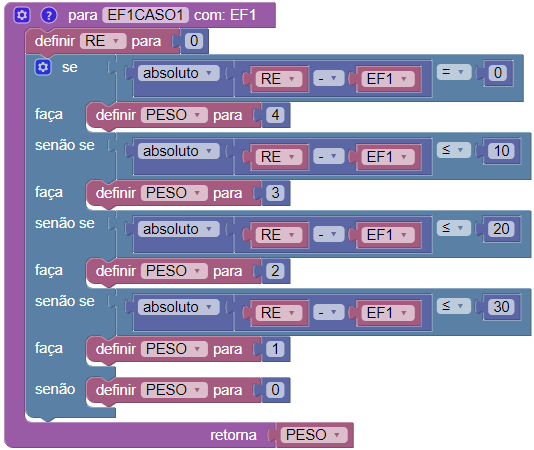
\includegraphics[width=0.6\linewidth]{chapters/appendixAnalytics/CASO1NPEF1.png}  \end{tabular}
%		} & \begin{tabular}[c]{@{}l@{}}import math \\ \# Nota Ponderada - Caso 1\\ def EF1CASO1(EF1):\\ \quad global RE, PESO\\ \quad RE = 0\\ \quad	if math.fabs(RE - EF1) == 0:\\	\quad \quad PESO = 4\\ \quad elif math.fabs(RE - EF1) <= 10:\\ \quad \quad PESO = 3\\	\quad elif math.fabs(RE - EF1) <= 20:\\ \quad \quad	PESO = 2\\ \quad elif math.fabs(RE - EF1) <= 30:\\ \quad \quad PESO = 1\\ \quad	else:\\ \quad \quad	PESO = 0\\ \quad return PESO
%		\end{tabular}  \\ \hline
%	\end{tabular}
%\end{table}
%
%\begin{table}[htb!]
%	\caption{Nota Ponderada - Caso de Teste 1 - EV1}
%	\centering
%	\begin{tabular}{|c|c|}
%		\hline
%		\multicolumn{2}{|c|}{\cellcolor[HTML]{DEDEDE}\textbf{NP - CASO 1 - EV1}} \\ \hline
%		\textbf{Blocos} & \multicolumn{1}{c|}{\textbf{Python gerado}} \\ \hline
%		\multicolumn{1}{|l|}{\begin{tabular}[c]{@{}l@{}} \\ 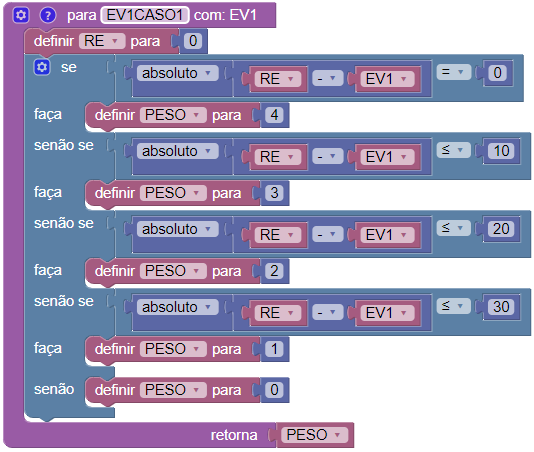
\includegraphics[width=0.6\linewidth]{chapters/appendixAnalytics/CASO1NPEV1.png}  \end{tabular}
%		} & \begin{tabular}[c]{@{}l@{}}import math \\ \# Nota Ponderada - Caso 1\\ def EV1CASO1(EV1):\\ \quad global RE, PESO\\ \quad RE = 0\\ \quad	if math.fabs(RE - EV1) == 0:\\	\quad \quad PESO = 4\\ \quad elif math.fabs(RE - EV1) <= 10:\\ \quad \quad PESO = 3\\	\quad elif math.fabs(RE - EV1) <= 20:\\ \quad \quad	PESO = 2\\ \quad elif math.fabs(RE - EV1) <= 30:\\ \quad \quad PESO = 1\\ \quad	else:\\ \quad \quad	PESO = 0\\ \quad return PESO
%		\end{tabular}  \\ \hline
%	\end{tabular}
%\end{table}
%
%\begin{table}[htb!]
%	\caption{Nota Ponderada - Caso de Teste 1 - EV2}
%	\centering
%	\begin{tabular}{|c|c|}
%		\hline
%		\multicolumn{2}{|c|}{\cellcolor[HTML]{DEDEDE}\textbf{NP - CASO 1 - EV2}} \\ \hline
%		\textbf{Blocos} & \multicolumn{1}{c|}{\textbf{Python gerado}} \\ \hline
%		\multicolumn{1}{|l|}{\begin{tabular}[c]{@{}l@{}} \\ 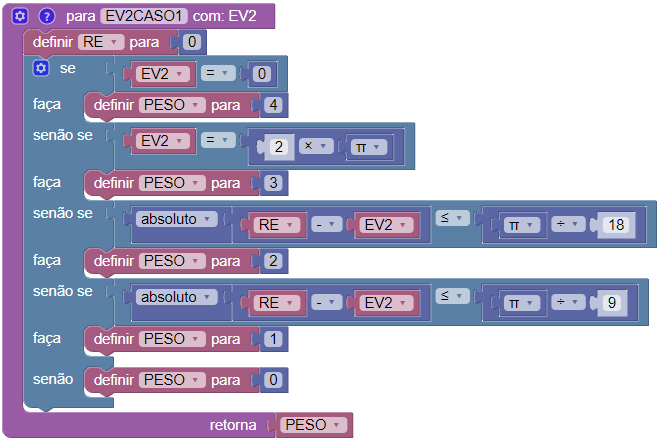
\includegraphics[width=0.6\linewidth]{chapters/appendixAnalytics/CASO1NPEV2.png}  \end{tabular}
%		} & \begin{tabular}[c]{@{}l@{}}import math\\ \# Nota Ponderada - Caso 1\\  def EV2CASO1(EV2):\\ \quad	global RE, PESO\\ \quad	RE = 0\\ \quad if EV2 == 0:\\ \quad \quad PESO = 4\\ \quad elif EV2 == 2 * math.pi:\\ \quad \quad	PESO = 3\\ \quad elif math.fabs(RE - EV2) <= math.pi / 18:\\ \quad \quad	PESO = 2\\ \quad	elif math.fabs(RE - EV2) <= math.pi / 9:\\ \quad \quad	PESO = 1\\ \quad	else:\\ \quad \quad		PESO = 0\\ \quad return PESO
%		\end{tabular}  \\ \hline
%	\end{tabular}
%\end{table}

%%CASO 2
%\begin{table}[htb!]
%	\caption{Nota Ponderada - Caso de Teste 2 - EF1}
%	\centering
%	\begin{tabular}{|c|c|}
%		\hline
%		\multicolumn{2}{|c|}{\cellcolor[HTML]{DEDEDE}\textbf{NP - CASO 2 - EF1}} \\ \hline
%		\textbf{Blocos} & \multicolumn{1}{c|}{\textbf{Python gerado}} \\ \hline
%		\multicolumn{1}{|l|}{\begin{tabular}[c]{@{}l@{}} \\ 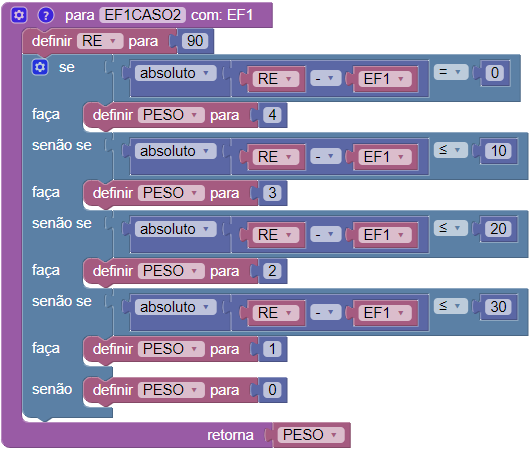
\includegraphics[width=0.6\linewidth]{chapters/appendixAnalytics/CASO2NPEF1.png}  \end{tabular}
%		} & \begin{tabular}[c]{@{}l@{}}import math \\ \# Nota Ponderada - Caso 2\\ def EF1CASO2(EF1):\\ \quad global RE, PESO\\ \quad RE = 90\\ \quad	if math.fabs(RE - EF1) == 0:\\	\quad \quad PESO = 4\\ \quad elif math.fabs(RE - EF1) <= 10:\\ \quad \quad PESO = 3\\	\quad elif math.fabs(RE - EF1) <= 20:\\ \quad \quad	PESO = 2\\ \quad elif math.fabs(RE - EF1) <= 30:\\ \quad \quad PESO = 1\\ \quad	else:\\ \quad \quad	PESO = 0\\ \quad return PESO
%		\end{tabular}  \\ \hline
%	\end{tabular}
%\end{table}
%
%\begin{table}[htb!]
%	\caption{Nota Ponderada - Caso de Teste 2 - EV1}
%	\centering
%	\begin{tabular}{|c|c|}
%		\hline
%		\multicolumn{2}{|c|}{\cellcolor[HTML]{DEDEDE}\textbf{NP - CASO 2 - EV1}} \\ \hline
%		\textbf{Blocos} & \multicolumn{1}{c|}{\textbf{Python gerado}} \\ \hline
%		\multicolumn{1}{|l|}{\begin{tabular}[c]{@{}l@{}} \\ 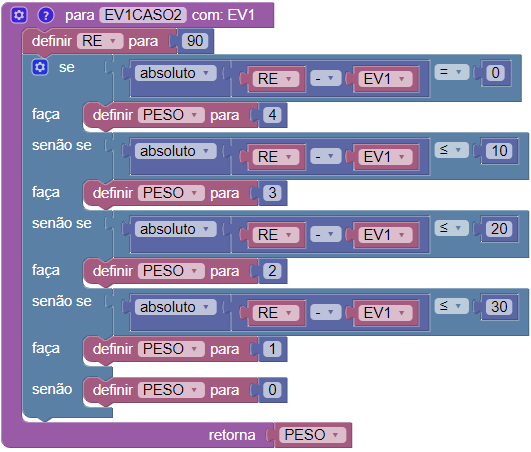
\includegraphics[width=0.6\linewidth]{chapters/appendixAnalytics/CASO2NPEV1.png}  \end{tabular}
%		} & \begin{tabular}[c]{@{}l@{}}import math \\ \# Nota Ponderada - Caso 1\\ def EV1CASO2(EV1):\\ \quad global RE, PESO\\ \quad RE = 90\\ \quad	if math.fabs(RE - EV1) == 0:\\	\quad \quad PESO = 4\\ \quad elif math.fabs(RE - EV1) <= 10:\\ \quad \quad PESO = 3\\	\quad elif math.fabs(RE - EV1) <= 20:\\ \quad \quad	PESO = 2\\ \quad elif math.fabs(RE - EV1) <= 30:\\ \quad \quad PESO = 1\\ \quad	else:\\ \quad \quad	PESO = 0\\ \quad return PESO
%		\end{tabular}  \\ \hline
%	\end{tabular}
%\end{table}
%
%\begin{table}[htb!]
%	\caption{Nota Ponderada - Caso de Teste 2 - EV2}
%	\centering
%	\begin{tabular}{|c|c|}
%		\hline
%		\multicolumn{2}{|c|}{\cellcolor[HTML]{DEDEDE}\textbf{NP - CASO 2 - EV2}} \\ \hline
%		\textbf{Blocos} & \multicolumn{1}{c|}{\textbf{Python gerado}} \\ \hline
%		\multicolumn{1}{|l|}{\begin{tabular}[c]{@{}l@{}} \\ 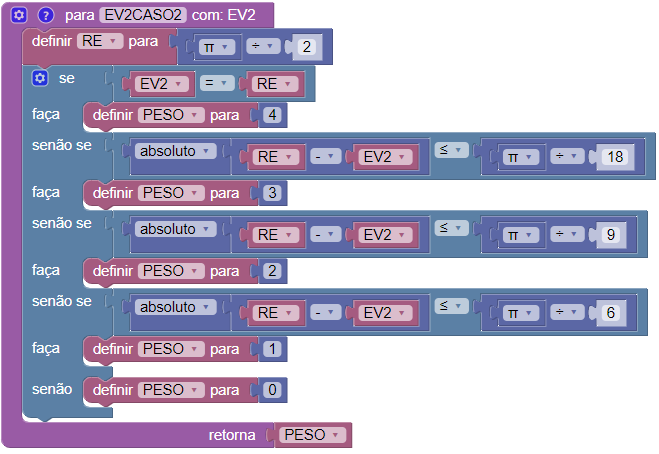
\includegraphics[width=0.6\linewidth]{chapters/appendixAnalytics/CASO2NPEV2.png}  \end{tabular}
%		} & \begin{tabular}[c]{@{}l@{}}import math\\ \# Nota Ponderada - Caso 2\\ def EV2CASO2(EV2):\\ \quad global RE, PESO\\ \quad RE = math.pi / 2\\ \quad if EV2 == RE:\\ \quad \quad PESO = 4\\ \quad elif math.fabs(RE - EV2) <= math.pi / 18:\\ \quad \quad PESO = 3\\ \quad elif math.fabs(RE - EV2) <= math.pi / 9:\\ \quad \quad PESO = 2\\ \quad elif math.fabs(RE - EV2) <= math.pi / 6:\\ \quad \quad PESO = 1\\ \quad else:\\ \quad \quad PESO = 0\\ \quad return PESO
%		\end{tabular}  \\ \hline
%	\end{tabular}
%\end{table}

%%CASO 3
%\begin{table}[htb!]
%	\caption{Nota Ponderada - Caso de Teste 3 - EF1}
%	\centering
%	\begin{tabular}{|c|c|}
%		\hline
%		\multicolumn{2}{|c|}{\cellcolor[HTML]{DEDEDE}\textbf{NP - CASO 3 - EF1}} \\ \hline
%		\textbf{Blocos} & \multicolumn{1}{c|}{\textbf{Python gerado}} \\ \hline
%		\multicolumn{1}{|l|}{\begin{tabular}[c]{@{}l@{}} \\ 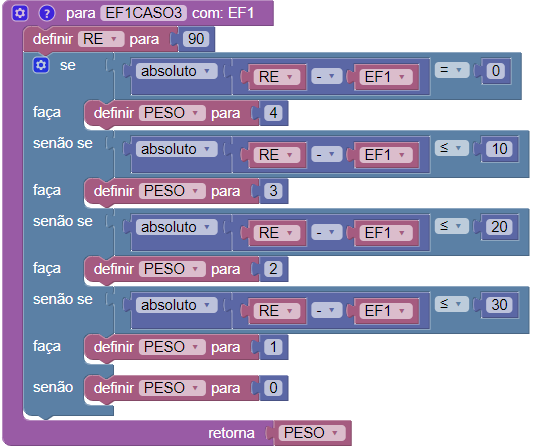
\includegraphics[width=0.6\linewidth]{chapters/appendixAnalytics/CASO3NPEF1.png}  \end{tabular}
%		} & \begin{tabular}[c]{@{}l@{}}import math \\ \# Nota Ponderada - Caso 3\\ def EF1CASO3(EF1):\\ \quad global RE, PESO\\ \quad RE = 90\\ \quad	if math.fabs(RE - EF1) == 0:\\	\quad \quad PESO = 4\\ \quad elif math.fabs(RE - EF1) <= 10:\\ \quad \quad PESO = 3\\	\quad elif math.fabs(RE - EF1) <= 20:\\ \quad \quad	PESO = 2\\ \quad elif math.fabs(RE - EF1) <= 30:\\ \quad \quad PESO = 1\\ \quad	else:\\ \quad \quad	PESO = 0\\ \quad return PESO
%		\end{tabular}  \\ \hline
%	\end{tabular}
%\end{table}
%
%\begin{table}[htb!]
%	\caption{Nota Ponderada - Caso de Teste 3 - EV1}
%	\centering
%	\begin{tabular}{|c|c|}
%		\hline
%		\multicolumn{2}{|c|}{\cellcolor[HTML]{DEDEDE}\textbf{NP - CASO 3 - EV1}} \\ \hline
%		\textbf{Blocos} & \multicolumn{1}{c|}{\textbf{Python gerado}} \\ \hline
%		\multicolumn{1}{|l|}{\begin{tabular}[c]{@{}l@{}} \\ 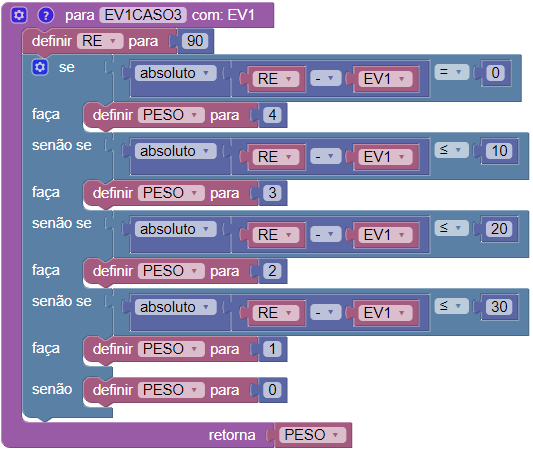
\includegraphics[width=0.6\linewidth]{chapters/appendixAnalytics/CASO3NPEV1.png}  \end{tabular}
%		} & \begin{tabular}[c]{@{}l@{}}import math \\ \# Nota Ponderada - Caso 3\\ def EV1CASO3(EV1):\\ \quad global RE, PESO\\ \quad RE = 90\\ \quad	if math.fabs(RE - EV1) == 0:\\	\quad \quad PESO = 4\\ \quad elif math.fabs(RE - EV1) <= 10:\\ \quad \quad PESO = 3\\	\quad elif math.fabs(RE - EV1) <= 20:\\ \quad \quad	PESO = 2\\ \quad elif math.fabs(RE - EV1) <= 30:\\ \quad \quad PESO = 1\\ \quad	else:\\ \quad \quad	PESO = 0\\ \quad return PESO
%		\end{tabular}  \\ \hline
%	\end{tabular}
%\end{table}
%
%\begin{table}[htb!]
%	\caption{Nota Ponderada - Caso de Teste 3 - EV2}
%	\centering
%	\begin{tabular}{|c|c|}
%		\hline
%		\multicolumn{2}{|c|}{\cellcolor[HTML]{DEDEDE}\textbf{NP - CASO 3 - EV2}} \\ \hline
%		\textbf{Blocos} & \multicolumn{1}{c|}{\textbf{Python gerado}} \\ \hline
%		\multicolumn{1}{|l|}{\begin{tabular}[c]{@{}l@{}} \\ 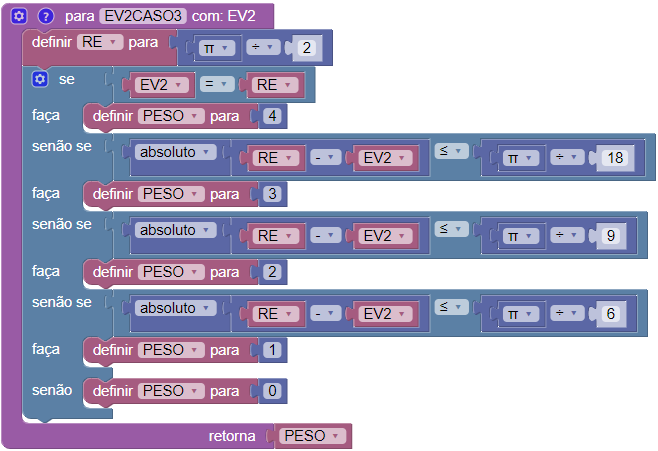
\includegraphics[width=0.6\linewidth]{chapters/appendixAnalytics/CASO3NPEV2.png}  \end{tabular}
%		} & \begin{tabular}[c]{@{}l@{}}import math\\ \# Nota Ponderada - EV2 - Caso 3\\ def EV2CASO3(EV2):\\ \quad	global RE, PESO\\ \quad RE = math.pi / 2\\ if EV2 == RE:\\ \quad 	PESO = 4\\ \quad elif math.fabs(RE - EV2) <= math.pi / 18:\\ \quad \quad PESO = 3\\ \quad elif math.fabs(RE - EV2) <= math.pi / 9:\\ \quad \quad PESO = 2\\ \quad elif math.fabs(RE - EV2) <= math.pi / 6:\\ \quad \quad PESO = 1\\ \quad	else:\\ \quad \quad PESO = 0\\ \quad return PESO
%		\end{tabular}  \\ \hline
%	\end{tabular}
%\end{table}

%%CASO 4
%\begin{table}[htb!]
%	\caption{Nota Ponderada - Caso de Teste 4 - EF1}
%	\centering
%	\begin{tabular}{|c|c|}
%		\hline
%		\multicolumn{2}{|c|}{\cellcolor[HTML]{DEDEDE}\textbf{NP - CASO 4 - EF1}} \\ \hline
%		\textbf{Blocos} & \multicolumn{1}{c|}{\textbf{Python gerado}} \\ \hline
%		\multicolumn{1}{|l|}{\begin{tabular}[c]{@{}l@{}} \\ 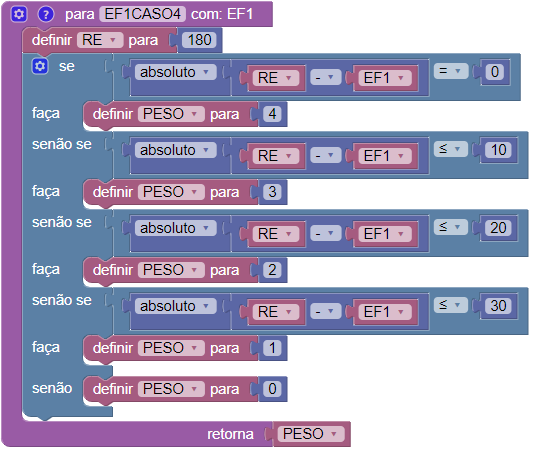
\includegraphics[width=0.6\linewidth]{chapters/appendixAnalytics/CASO4NPEF1.png}  \end{tabular}
%		} & \begin{tabular}[c]{@{}l@{}}import math \\ \# Nota Ponderada - Caso 4\\ def EF1CASO4(EF1):\\ \quad global RE, PESO\\ \quad RE = 180\\ \quad	if math.fabs(RE - EF1) == 0:\\	\quad \quad PESO = 4\\ \quad elif math.fabs(RE - EF1) <= 10:\\ \quad \quad PESO = 3\\	\quad elif math.fabs(RE - EF1) <= 20:\\ \quad \quad	PESO = 2\\ \quad elif math.fabs(RE - EF1) <= 30:\\ \quad \quad PESO = 1\\ \quad	else:\\ \quad \quad	PESO = 0\\ \quad return PESO
%		\end{tabular}  \\ \hline
%	\end{tabular}
%\end{table}
%
%\begin{table}[htb!]
%	\caption{Nota Ponderada - Caso de Teste 3 - EV1}
%	\centering
%	\begin{tabular}{|c|c|}
%		\hline
%		\multicolumn{2}{|c|}{\cellcolor[HTML]{DEDEDE}\textbf{NP - CASO 4 - EV1}} \\ \hline
%		\textbf{Blocos} & \multicolumn{1}{c|}{\textbf{Python gerado}} \\ \hline
%		\multicolumn{1}{|l|}{\begin{tabular}[c]{@{}l@{}} \\ 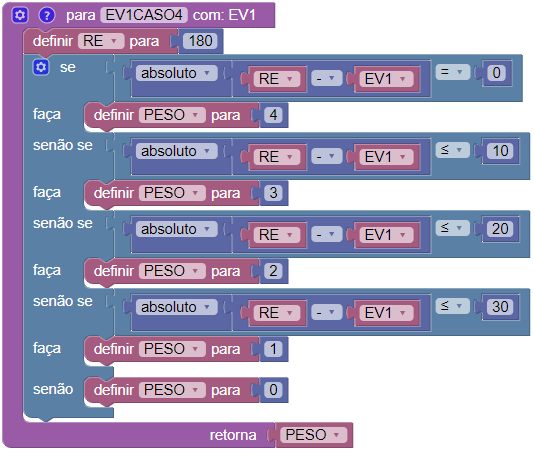
\includegraphics[width=0.6\linewidth]{chapters/appendixAnalytics/CASO4NPEV1.png}  \end{tabular}
%		} & \begin{tabular}[c]{@{}l@{}}import math \\ \# Nota Ponderada - Caso 4\\ def EV1CASO4(EV1):\\ \quad global RE, PESO\\ \quad RE = 180\\ \quad	if math.fabs(RE - EV1) == 0:\\	\quad \quad PESO = 4\\ \quad elif math.fabs(RE - EV1) <= 10:\\ \quad \quad PESO = 3\\	\quad elif math.fabs(RE - EV1) <= 20:\\ \quad \quad	PESO = 2\\ \quad elif math.fabs(RE - EV1) <= 30:\\ \quad \quad PESO = 1\\ \quad	else:\\ \quad \quad	PESO = 0\\ \quad return PESO
%		\end{tabular}  \\ \hline
%	\end{tabular}
%\end{table}
%
%\begin{table}[htb!]
%	\caption{Nota Ponderada - Caso de Teste 4 - EV2}
%	\centering
%	\begin{tabular}{|c|c|}
%		\hline
%		\multicolumn{2}{|c|}{\cellcolor[HTML]{DEDEDE}\textbf{NP - CASO 4 - EV2}} \\ \hline
%		\textbf{Blocos} & \multicolumn{1}{c|}{\textbf{Python gerado}} \\ \hline
%		\multicolumn{1}{|l|}{\begin{tabular}[c]{@{}l@{}} \\ 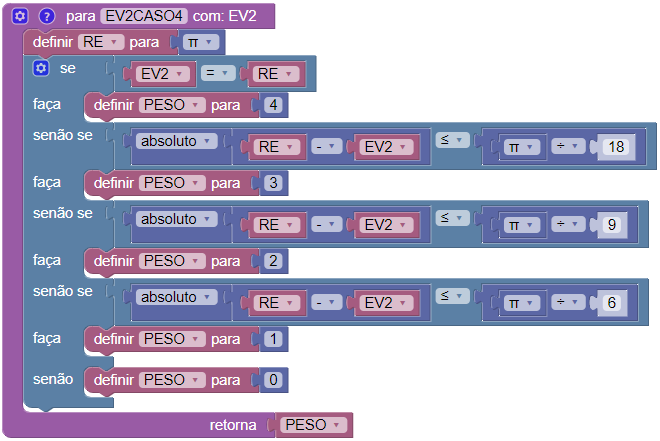
\includegraphics[width=0.6\linewidth]{chapters/appendixAnalytics/CASO4NPEV2.png}  \end{tabular}
%		} & \begin{tabular}[c]{@{}l@{}}import math \\ \# Nota Ponderada - EV2 - Caso 4\\ def EV2CASO4(EV2):\\ \quad global RE, PESO \\ \quad RE = math.pi \\ \quad if EV2 == RE:\\ \quad \quad	PESO = 4\\ \quad	elif math.fabs(RE - EV2) <= math.pi / 18:\\ \quad \quad PESO = 3\\ \quad	elif math.fabs(RE - EV2) <= math.pi / 9:\\ \quad \quad	PESO = 2\\ \quad	elif math.fabs(RE - EV2) <= math.pi / 6:\\ \quad \quad PESO = 1\\ \quad	else: \\ \quad \quad	PESO = 0\\ \quad return PESO
%		\end{tabular}  \\ \hline
%	\end{tabular}
%\end{table}

%%CASO 5
%\begin{table}[htb!]
%	\caption{Nota Ponderada - Caso de Teste 5 - EF1}
%	\centering
%	\begin{tabular}{|c|c|}
%		\hline
%		\multicolumn{2}{|c|}{\cellcolor[HTML]{DEDEDE}\textbf{NP - CASO 5 - EF1}} \\ \hline
%		\textbf{Blocos} & \multicolumn{1}{c|}{\textbf{Python gerado}} \\ \hline
%		\multicolumn{1}{|l|}{\begin{tabular}[c]{@{}l@{}} \\ 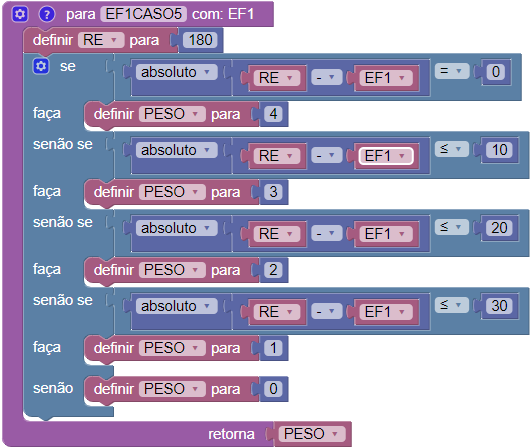
\includegraphics[width=0.6\linewidth]{chapters/appendixAnalytics/CASO5NPEF1.png}  \end{tabular}
%		} & \begin{tabular}[c]{@{}l@{}}import math \\ \# Nota Ponderada - Caso 5\\ def EF1CASO5(EF1):\\ \quad global RE, PESO\\ \quad RE = 180\\ \quad	if math.fabs(RE - EF1) == 0:\\	\quad \quad PESO = 4\\ \quad elif math.fabs(RE - EF1) <= 10:\\ \quad \quad PESO = 3\\	\quad elif math.fabs(RE - EF1) <= 20:\\ \quad \quad	PESO = 2\\ \quad elif math.fabs(RE - EF1) <= 30:\\ \quad \quad PESO = 1\\ \quad	else:\\ \quad \quad	PESO = 0\\ \quad return PESO
%		\end{tabular}  \\ \hline
%	\end{tabular}
%\end{table}
%
%\begin{table}[htb!]
%	\caption{Nota Ponderada - Caso de Teste 5 - EV1}
%	\centering
%	\begin{tabular}{|c|c|}
%		\hline
%		\multicolumn{2}{|c|}{\cellcolor[HTML]{DEDEDE}\textbf{NP - CASO 5 - EV1}} \\ \hline
%		\textbf{Blocos} & \multicolumn{1}{c|}{\textbf{Python gerado}} \\ \hline
%		\multicolumn{1}{|l|}{\begin{tabular}[c]{@{}l@{}} \\ 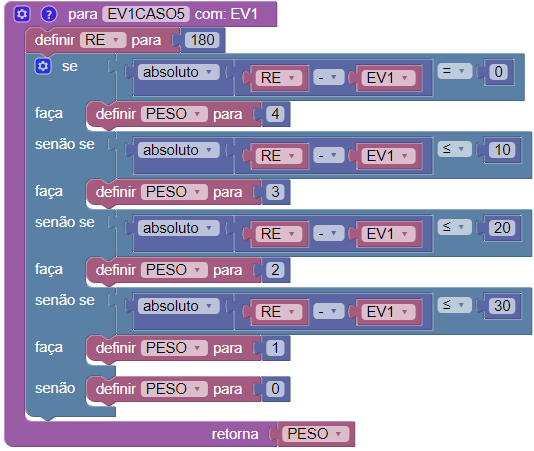
\includegraphics[width=0.6\linewidth]{chapters/appendixAnalytics/CASO5NPEV1.png}  \end{tabular}
%		} & \begin{tabular}[c]{@{}l@{}}import math \\ \# Nota Ponderada - Caso 5\\ def EV1CASO5(EV1):\\ \quad global RE, PESO\\ \quad RE = 180\\ \quad	if math.fabs(RE - EV1) == 0:\\	\quad \quad PESO = 4\\ \quad elif math.fabs(RE - EV1) <= 10:\\ \quad \quad PESO = 3\\	\quad elif math.fabs(RE - EV1) <= 20:\\ \quad \quad	PESO = 2\\ \quad elif math.fabs(RE - EV1) <= 30:\\ \quad \quad PESO = 1\\ \quad	else:\\ \quad \quad	PESO = 0\\ \quad return PESO
%		\end{tabular}  \\ \hline
%	\end{tabular}
%\end{table}
%
%\begin{table}[htb!]
%	\caption{Nota Ponderada - Caso de Teste 5 - EV2}
%	\centering
%	\begin{tabular}{|c|c|}
%		\hline
%		\multicolumn{2}{|c|}{\cellcolor[HTML]{DEDEDE}\textbf{NP - CASO 5 - EV2}} \\ \hline
%		\textbf{Blocos} & \multicolumn{1}{c|}{\textbf{Python gerado}} \\ \hline
%		\multicolumn{1}{|l|}{\begin{tabular}[c]{@{}l@{}} \\ 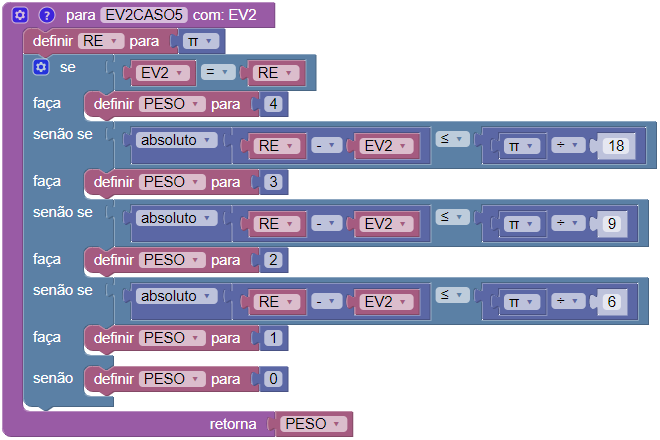
\includegraphics[width=0.6\linewidth]{chapters/appendixAnalytics/CASO5NPEV2.png}  \end{tabular}
%		} & \begin{tabular}[c]{@{}l@{}}import math\\ \# Nota Ponderada - EV2 - Caso 5\\ def EV2CASO5(EV2):\\ \quad	global RE, PESO\\ \quad RE = math.pi\\ \quad if EV2 == RE:\\ \quad \quad PESO = 4\\ \quad elif math.fabs(RE - EV2) <= math.pi / 18:\\ \quad \quad PESO = 3\\ \quad elif math.fabs(RE - EV2) <= math.pi / 9:\\ \quad \quad PESO = 2\\ \quad elif math.fabs(RE - EV2) <= math.pi / 6:\\ \quad \quad PESO = 1\\ \quad else:\\ \quad \quad PESO = 0\\ \quad return PESO
%		\end{tabular}  \\ \hline
%	\end{tabular}
%\end{table}

%%CASO 6
%\begin{table}[htb!]
%	\caption{Nota Ponderada - Caso de Teste 6 - EF1}
%	\centering
%	\begin{tabular}{|c|c|}
%		\hline
%		\multicolumn{2}{|c|}{\cellcolor[HTML]{DEDEDE}\textbf{NP - CASO 6 - EF1}} \\ \hline
%		\textbf{Blocos} & \multicolumn{1}{c|}{\textbf{Python gerado}} \\ \hline
%		\multicolumn{1}{|l|}{\begin{tabular}[c]{@{}l@{}} \\ 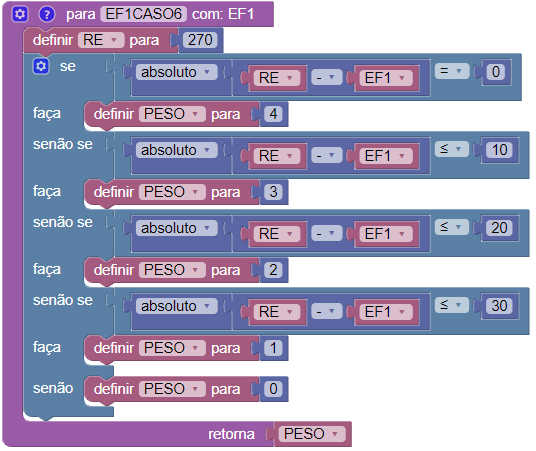
\includegraphics[width=0.6\linewidth]{chapters/appendixAnalytics/CASO6NPEF1.png}  \end{tabular}
%		} & \begin{tabular}[c]{@{}l@{}}import math \\ \# Nota Ponderada - Caso 6\\ def EF1CASO6(EF1):\\ \quad global RE, PESO\\ \quad RE = 270\\ \quad	if math.fabs(RE - EF1) == 0:\\	\quad \quad PESO = 4\\ \quad elif math.fabs(RE - EF1) <= 10:\\ \quad \quad PESO = 3\\	\quad elif math.fabs(RE - EF1) <= 20:\\ \quad \quad	PESO = 2\\ \quad elif math.fabs(RE - EF1) <= 30:\\ \quad \quad PESO = 1\\ \quad	else:\\ \quad \quad	PESO = 0\\ \quad return PESO
%		\end{tabular}  \\ \hline
%	\end{tabular}
%\end{table}
%
%\begin{table}[htb!]
%	\caption{Nota Ponderada - Caso de Teste 6 - EV1}
%	\centering
%	\begin{tabular}{|c|c|}
%		\hline
%		\multicolumn{2}{|c|}{\cellcolor[HTML]{DEDEDE}\textbf{NP - CASO 6 - EV1}} \\ \hline
%		\textbf{Blocos} & \multicolumn{1}{c|}{\textbf{Python gerado}} \\ \hline
%		\multicolumn{1}{|l|}{\begin{tabular}[c]{@{}l@{}} \\ 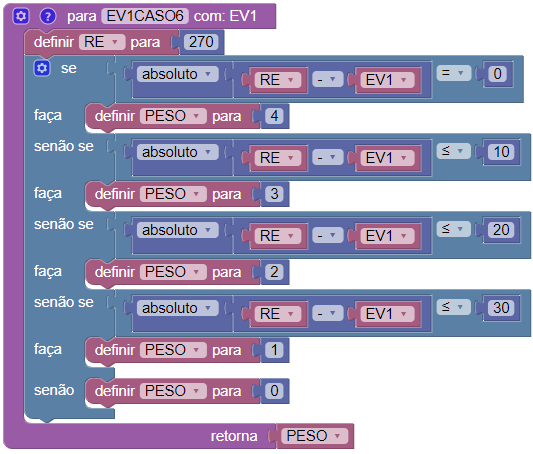
\includegraphics[width=0.6\linewidth]{chapters/appendixAnalytics/CASO6NPEV1.png}  \end{tabular}
%		} & \begin{tabular}[c]{@{}l@{}}import math \\ \# Nota Ponderada - Caso 6\\ def EV1CASO6(EV1):\\ \quad global RE, PESO\\ \quad RE = 270\\ \quad	if math.fabs(RE - EV1) == 0:\\	\quad \quad PESO = 4\\ \quad elif math.fabs(RE - EV1) <= 10:\\ \quad \quad PESO = 3\\	\quad elif math.fabs(RE - EV1) <= 20:\\ \quad \quad	PESO = 2\\ \quad elif math.fabs(RE - EV1) <= 30:\\ \quad \quad PESO = 1\\ \quad	else:\\ \quad \quad	PESO = 0\\ \quad return PESO
%		\end{tabular}  \\ \hline
%	\end{tabular}
%\end{table}
%
%\begin{table}[htb!]
%	\caption{Nota Ponderada - Caso de Teste 6 - EV2}
%	\centering
%	\begin{tabular}{|c|c|}
%		\hline
%		\multicolumn{2}{|c|}{\cellcolor[HTML]{DEDEDE}\textbf{NP - CASO 6 - EV2}} \\ \hline
%		\textbf{Blocos} & \multicolumn{1}{c|}{\textbf{Python gerado}} \\ \hline
%		\multicolumn{1}{|l|}{\begin{tabular}[c]{@{}l@{}} \\ 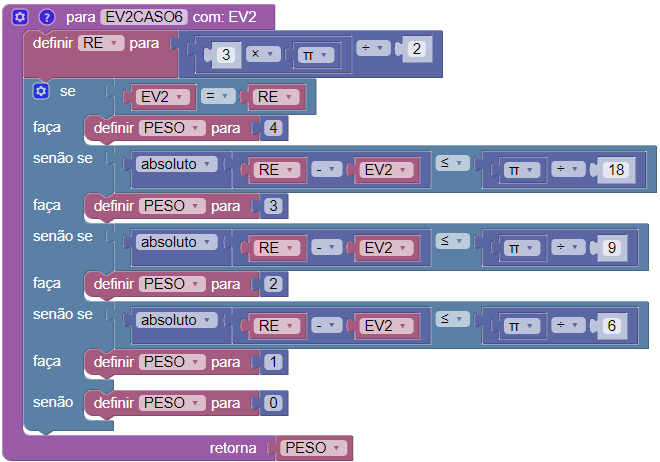
\includegraphics[width=0.6\linewidth]{chapters/appendixAnalytics/CASO6NPEV2.png}  \end{tabular}
%		} & \begin{tabular}[c]{@{}l@{}}import math \\ \# Nota Ponderada - EV2 - Caso 6\\ def EV2CASO6(EV2):\\ \quad global RE, PESO \\ \quad RE = (3 * math.pi) / 2 \\ \quad if EV2 == RE:\\ \quad \quad	PESO = 4\\ \quad	elif math.fabs(RE - EV2) <= math.pi / 18:\\ \quad \quad PESO = 3\\ \quad	elif math.fabs(RE - EV2) <= math.pi / 9:\\ \quad \quad	PESO = 2\\ \quad	elif math.fabs(RE - EV2) <= math.pi / 6:\\ \quad \quad PESO = 1\\ \quad	else: \\ \quad \quad	PESO = 0\\ \quad return PESO
%		\end{tabular}  \\ \hline
%	\end{tabular}
%\end{table}

%%CASO 7
%\begin{table}[htb!]
%	\caption{Nota Ponderada - Caso de Teste 7 - EF1}
%	\centering
%	\begin{tabular}{|c|c|}
%		\hline
%		\multicolumn{2}{|c|}{\cellcolor[HTML]{DEDEDE}\textbf{NP - CASO 7 - EF1}} \\ \hline
%		\textbf{Blocos} & \multicolumn{1}{c|}{\textbf{Python gerado}} \\ \hline
%		\multicolumn{1}{|l|}{\begin{tabular}[c]{@{}l@{}} \\ 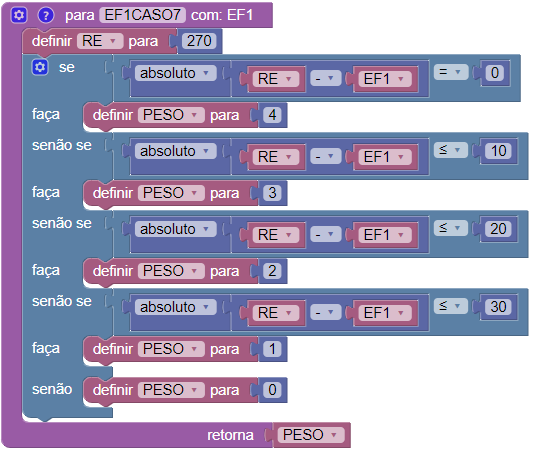
\includegraphics[width=0.6\linewidth]{chapters/appendixAnalytics/CASO7NPEF1.png}  \end{tabular}
%		} & \begin{tabular}[c]{@{}l@{}}import math\\ \# Nota Ponderada - EF1 - Caso 7\\ def EF1CASO7(EF1):\\ \quad global RE, PESO\\ \quad  RE = 270\\ \quad if math.fabs(RE - EF1) == 0:\\ \quad \quad PESO = 4\\ \quad elif math.fabs(RE - EF1) <= 10:\\ \quad \quad PESO = 3\\ \quad elif math.fabs(RE - EF1) <= 20:\\ \quad \quad PESO = 2\\ \quad elif math.fabs(RE - EF1) <= 30:\\ \quad \quad PESO = 1\\ \quad else:\\ \quad \quad PESO = 0\\ \quad return PESO		
%		\end{tabular}  \\ \hline
%	\end{tabular}
%\end{table}
%
%\begin{table}[htb!]
%	\caption{Nota Ponderada - Caso de Teste 7 - EV1}
%	\centering
%	\begin{tabular}{|c|c|}
%		\hline
%		\multicolumn{2}{|c|}{\cellcolor[HTML]{DEDEDE}\textbf{NP - CASO 7 - EV1}} \\ \hline
%		\textbf{Blocos} & \multicolumn{1}{c|}{\textbf{Python gerado}} \\ \hline
%		\multicolumn{1}{|l|}{\begin{tabular}[c]{@{}l@{}} \\ 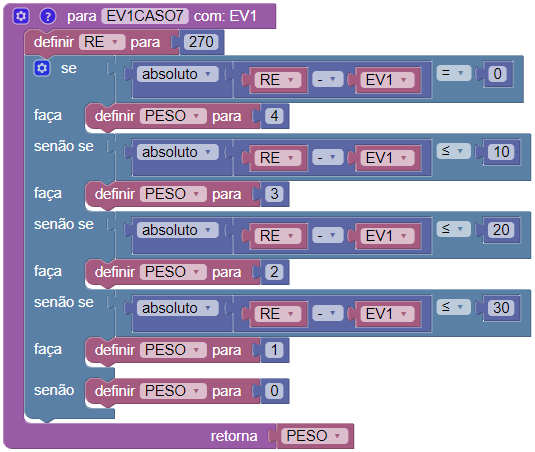
\includegraphics[width=0.6\linewidth]{chapters/appendixAnalytics/CASO7NPEV1.png}  \end{tabular}
%		} & \begin{tabular}[c]{@{}l@{}}import math \\ \# Nota Ponderada - EV1 - Caso 7\\ def EV1CASO7(EV1):\\ \quad global RE, PESO\\ \quad RE = 270\\ \quad if math.fabs(RE - EV1) == 0:\\ \quad \quad PESO = 4\\ \quad elif math.fabs(RE - EV1) <= 10:\\ \quad \quad PESO = 3\\ \quad elif math.fabs(RE - EV1) <= 20:\\ \quad \quad PESO = 2\\ \quad elif math.fabs(RE - EV1) <= 30:\\ \quad \quad PESO = 1\\ \quad else:\\ \quad \quad PESO = 0\\ \quad return PESO
%		\end{tabular}  \\ \hline
%	\end{tabular}
%\end{table}
%
%\begin{table}[htb!]
%	\caption{Nota Ponderada - Caso de Teste 7 - EV2}
%	\centering
%	\begin{tabular}{|c|c|}
%		\hline
%		\multicolumn{2}{|c|}{\cellcolor[HTML]{DEDEDE}\textbf{NP - CASO 7 - EV2}} \\ \hline
%		\textbf{Blocos} & \multicolumn{1}{c|}{\textbf{Python gerado}} \\ \hline
%		\multicolumn{1}{|l|}{\begin{tabular}[c]{@{}l@{}} \\ 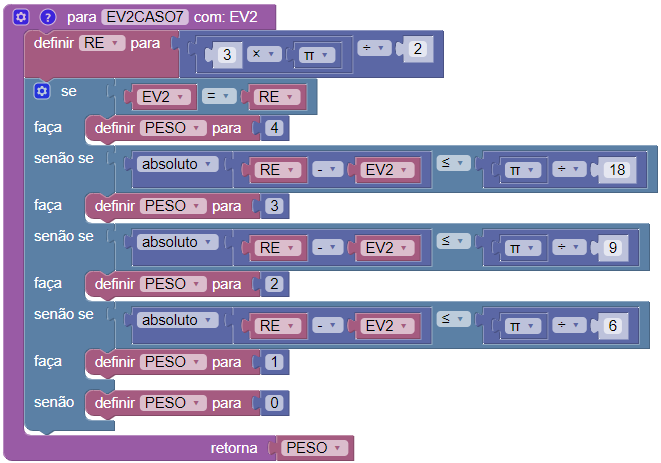
\includegraphics[width=0.6\linewidth]{chapters/appendixAnalytics/CASO7NPEV2.png}  \end{tabular}
%		} & \begin{tabular}[c]{@{}l@{}}import math \\ \# Nota Ponderada - EV2 - Caso 7\\ def EV2CASO7(EV2):\\ \quad global RE, PESO\\ \quad RE = (3 * math.pi) / 2\\ \quad if EV2 == RE:\\ \quad \quad PESO = 4\\ \quad elif math.fabs(RE - EV2) <= math.pi / 18:\\ \quad \quad PESO = 3\\ \quad elif math.fabs(RE - EV2) <= math.pi / 9:\\ \quad \quad PESO = 2\\ \quad elif math.fabs(RE - EV2) <= math.pi / 6: \\ \quad \quad PESO = 1\\ \quad else:\\ \quad \quad PESO = 0\\ \quad return PESO
%		\end{tabular}  \\ \hline
%	\end{tabular}
%\end{table}
%
%%CASO 8
%\begin{table}[htb!]
%	\caption{Nota Ponderada - Caso de Teste 8 - EF1}
%	\centering
%	\begin{tabular}{|c|c|}
%		\hline
%		\multicolumn{2}{|c|}{\cellcolor[HTML]{DEDEDE}\textbf{NP - CASO 8 - EF1}} \\ \hline
%		\textbf{Blocos} & \multicolumn{1}{c|}{\textbf{Python gerado}} \\ \hline
%		\multicolumn{1}{|l|}{\begin{tabular}[c]{@{}l@{}} \\ 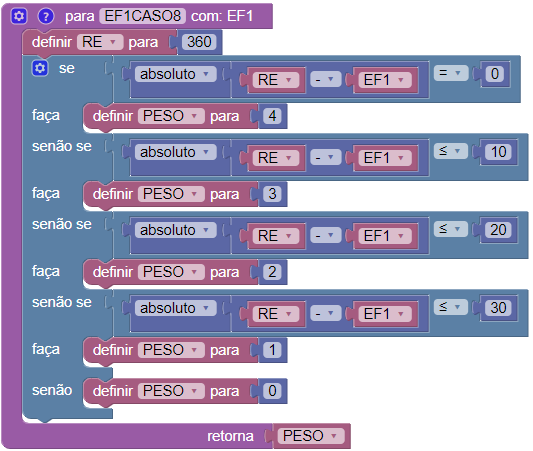
\includegraphics[width=0.6\linewidth]{chapters/appendixAnalytics/CASO8NPEF1.png}  \end{tabular}
%		} & \begin{tabular}[c]{@{}l@{}}import math\\ \# Nota Ponderada - EF1 - Caso 8\\ def EF1CASO8(EF1):\\ \quad global RE, PESO\\ \quad RE = 360\\ \quad if math.fabs(RE - EF1) == 0:\\ \quad \quad PESO = 4\\ \quad elif math.fabs(RE - EF1) <= 10:\\ \quad \quad PESO = 3\\ \quad elif math.fabs(RE - EF1) <= 20:\\ \quad \quad PESO = 2\\ \quad elif math.fabs(RE - EF1) <= 30:\\ \quad \quad PESO = 1\\ \quad else:\\ \quad \quad PESO = 0\\ \quad return PESO
%		\end{tabular}  \\ \hline
%	\end{tabular}
%\end{table}
%
%\begin{table}[htb!]
%	\caption{Nota Ponderada - Caso de Teste 8 - EV1}
%	\centering
%	\begin{tabular}{|c|c|}
%		\hline
%		\multicolumn{2}{|c|}{\cellcolor[HTML]{DEDEDE}\textbf{NP - CASO 8 - EV1}} \\ \hline
%		\textbf{Blocos} & \multicolumn{1}{c|}{\textbf{Python gerado}} \\ \hline
%		\multicolumn{1}{|l|}{\begin{tabular}[c]{@{}l@{}} \\ 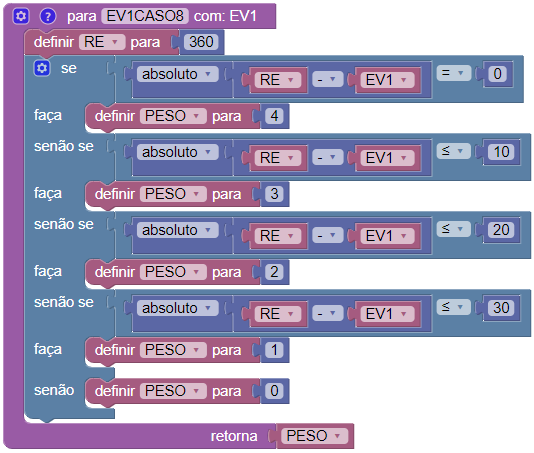
\includegraphics[width=0.6\linewidth]{chapters/appendixAnalytics/CASO8NPEV1.png}  \end{tabular}
%		} & \begin{tabular}[c]{@{}l@{}}import math \\ \# Nota Ponderada - EV1 - Caso 8\\ def EV1CASO8(EV1):\\ \quad global RE, PESO\\ \quad RE = 360\\ \quad if math.fabs(RE - EV1) == 0:\\ \quad \quad PESO = 4\\ \quad elif math.fabs(RE - EV1) <= 10:\\ \quad \quad PESO = 3\\ \quad elif math.fabs(RE - EV1) <= 20:\\ \quad \quad PESO = 2\\ \quad elif math.fabs(RE - EV1) <= 30:\\ \quad \quad PESO = 1\\ \quad else:\\ \quad \quad PESO = 0\\ \quad return PESO
%		\end{tabular}  \\ \hline
%	\end{tabular}
%\end{table}
%
%\begin{table}[htb!]
%	\caption{Nota Ponderada - Caso de Teste 8 - EV2}
%	\centering
%	\begin{tabular}{|c|c|}
%		\hline
%		\multicolumn{2}{|c|}{\cellcolor[HTML]{DEDEDE}\textbf{NP - CASO 8 - EV2}} \\ \hline
%		\textbf{Blocos} & \multicolumn{1}{c|}{\textbf{Python gerado}} \\ \hline
%		\multicolumn{1}{|l|}{\begin{tabular}[c]{@{}l@{}} \\ 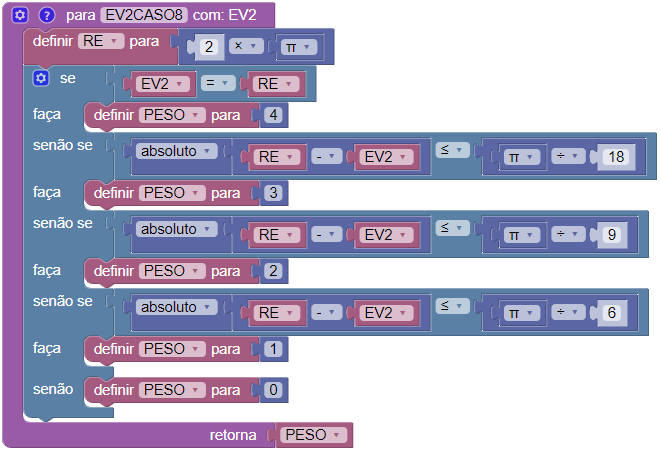
\includegraphics[width=0.6\linewidth]{chapters/appendixAnalytics/CASO8NPEV2.png}  \end{tabular}
%		} & \begin{tabular}[c]{@{}l@{}}import math \\ \# Nota Ponderada - EV2 - Caso 8\\ def EV2CASO8(EV2):\\ \quad global RE, PESO\\ \quad RE = 2 * math.pi\\ \quad if EV2 == RE:\\ \quad \quad PESO = 4\\ \quad elif math.fabs(RE - EV2) <= math.pi / 18:\\ \quad \quad PESO = 3\\ \quad elif math.fabs(RE - EV2) <= math.pi / 9:\\ \quad \quad PESO = 2\\ \quad elif math.fabs(RE - EV2) <= math.pi / 6:\\ \quad \quad PESO = 1\\ \quad else:\\ \quad \quad PESO = 0\\ \quad return PESO
%		\end{tabular}  \\ \hline
%	\end{tabular}
%\end{table}
